\documentclass[12pt,a4paper]{article}

% ================== 基本宏包 ==================
\usepackage{ctex} % 中文支持（推荐 XeLaTeX)
\usepackage{geometry}
\usepackage{amsmath,amssymb}
\usepackage{graphicx}
\usepackage{float}
\usepackage{booktabs}
\usepackage{hyperref}
\usepackage{listings}
\usepackage{xcolor}

\usepackage{microtype}

\tolerance=1000
\emergencystretch=3em

\geometry{left=2.5cm,right=2.5cm,top=2.8cm,bottom=2.8cm}
\setCJKmainfont[BoldFont=SimHei]{SimSun}


% ================== 代码样式 ==================
\lstset{
 basicstyle=\ttfamily\small,
 keywordstyle=\color{blue},
 commentstyle=\color{green!50!black},
 stringstyle=\color{red!60!black},
 numbers=left,
 numberstyle=\tiny,
 breaklines=true,
 frame=single,
 columns=flexible,
 showspaces=false,
 showstringspaces=false,
}

\title{\textbf{《数据可视化》结课作业} \\ \Large{Nyx宇宙学模拟的交互式可视分析与结构形成研究}}
\author{}
\date{\today}

\begin{document}
\maketitle
\tableofcontents
\newpage

%========================================
\section{数据处理过程}
%========================================

本研究基于 Nyx 宇宙学模拟程序生成的 100 个时间步、$128^3$ 分辨率的宇宙密度场数据开展分析。原始数据以二进制格式存储，每个时间步对应一个 \texttt{.dat} 文件，文件大小约为 8.4 MB，包含 $128 \times 128 \times 128 = 2\,097\,152$ 个 \texttt{float32} 小端序数值。由于数据文件未附带任何元数据头部，需要直接按原始字节流解析。具体而言，每个文件首先通过 Python 的 \texttt{open} 函数以二进制只读模式打开，读取全部字节后，利用 \texttt{struct.unpack} 配合格式字符串 \texttt{'<' + 'f' * n} 进行小端序浮点解析，其中 \texttt{'<'} 标记表示小端序，\texttt{'f'} 表示单精度浮点数。解析完成后，得到一维长度为 2,097,152 的数组，再通过 NumPy 的 \texttt{reshape((128, 128, 128))} 还原为三维张量，后续所有可视化分析均基于该张量进行。

\begin{lstlisting}[language=Python, caption=原始数据读取函数]
import struct, numpy as np

def read_raw_dat(filepath):
    with open(filepath, 'rb') as f:
        raw = f.read()
    n_floats = len(raw) // 4
    data = struct.unpack('<' + 'f' * n_floats, raw)
    return np.array(data, dtype=np.float32).reshape((128, 128, 128))
\end{lstlisting}

在获取三维密度场后，预处理流程按功能模块划分为五个独立的子数据处理步骤，每个步骤均面向后续特定的可视化需求，产出结构化的中间数据文件。

\paragraph{统计量计算}统计量计算面向任务二和任务四的时序演化分析需求，对每个时间步的 2,097,152 个密度值进行全局统计。具体而言，调用 NumPy 的 \texttt{data.min()}、\texttt{data.max()}、\texttt{data.mean()} 和 \texttt{data.std()} 获取最值与一阶矩，通过 \texttt{np.median(data.flatten())} 获取中位数，再通过 \texttt{np.percentile} 分别计算 P1、P5、P95、P99 和 P999 分位数。这些指标共同刻画了密度分布的整体位置、离散程度和尾部特征。计算完成后，将每个时间步的统计字典追加到列表，最终通过 \texttt{json.dump} 写入 \texttt{stats.json}，供后续所有图表统一读取。

\begin{lstlisting}[language=Python, caption=统计量计算关键代码]
def compute_stats(data):
    flat = data.flatten()
    return {
        'min': float(data.min()), 'max': float(data.max()),
        'mean': float(data.mean()), 'std': float(data.std()),
        'median': float(np.median(flat)),
        'p1': float(np.percentile(flat, 1)),
        'p5': float(np.percentile(flat, 5)),
        'p95': float(np.percentile(flat, 95)),
        'p99': float(np.percentile(flat, 99)),
        'p999': float(np.percentile(flat, 99.9)),
    }

# 主循环中批量写入
all_stats = []
for i in range(N_STEPS):
    data = load_timestep(i)
    stats = compute_stats(data)
    stats['timestep'] = i
    all_stats.append(stats)
with open(OUT_DIR / 'stats.json', 'w') as f:
    json.dump(all_stats, f)
\end{lstlisting}

\paragraph{原始密度直方图计算}原始密度直方图面向任务三的时序统计特征分析，直接在密度值域上进行 200 个等宽分箱统计。使用 \texttt{np.histogram(data.flatten(), bins=200, range=(data.min(), data.max()))} 计算频数数组和分箱边界数组，将两者转换为列表后存入字典。每个时间步的直方图数据包含时间步编号、频数序列和边界序列，最终全部写入 \texttt{histograms.json}。

\begin{lstlisting}[language=Python, caption=原始密度直方图计算关键代码]
def compute_histogram(data, bins=200):
    hist, edges = np.histogram(data.flatten(), bins=bins,
                               range=(data.min(), data.max()))
    return hist.tolist(), edges.tolist()

all_histograms = []
for i in range(N_STEPS):
    data = load_timestep(i)
    hist, edges = compute_histogram(data, bins=200)
    all_histograms.append({'timestep': i, 'hist': hist, 'edges': edges})
with open(OUT_DIR / 'histograms.json', 'w') as f:
    json.dump(all_histograms, f)
\end{lstlisting}

\paragraph{对数密度直方图计算}对数密度直方图面向任务三中压缩高密度动态范围的需求，先对密度值取 $\log_{10}$ 变换再分箱统计。具体实现为 \texttt{np.log10(data - data.min() + 1e-6)}，其中减去最小值并加上 $10^{-6}$ 确保非负性。变换后使用 \texttt{np.histogram} 进行 200 分箱统计，结果写入 \texttt{log\_histograms.json}。这种对数尺度处理使得低密度区域的空洞结构在直方图中清晰可辨，避免了原始尺度下高密度尾部掩盖低密度的现象。

\begin{lstlisting}[language=Python, caption=对数密度直方图计算关键代码]
def compute_histogram_log(data, bins=200):
    log_data = np.log10(data - data.min() + 1e-6)
    hist, edges = np.histogram(log_data.flatten(), bins=bins)
    return hist.tolist(), edges.tolist()

all_log_histograms = []
for i in range(N_STEPS):
    data = load_timestep(i)
    log_hist, log_edges = compute_histogram_log(data, bins=200)
    all_log_histograms.append({'timestep': i, 'hist': log_hist, 'edges': log_edges})
with open(OUT_DIR / 'log_histograms.json', 'w') as f:
    json.dump(all_log_histograms, f)
\end{lstlisting}

\paragraph{MIP 与 AIP 投影图生成}投影图生成面向任务一的二维空间结构展示和 Web 前端二维切面参考面板。对每个时间步，沿 X、Y、Z 三个轴分别计算最大强度投影（MIP）和平均强度投影（AIP）。MIP 使用 \texttt{np.max(data, axis)} 沿指定轴取最大值，突出高密度骨架；AIP 使用 \texttt{np.mean(data, axis)} 保留整体密度加权平均。Matplotlib 以 \texttt{cmap='hot'} 渲染并保存为 PNG 文件。关键时间步（0、25、50、75、99）的投影图同时用于报告插图和 Web 前端。

\begin{lstlisting}[language=Python, caption=MIP 与 AIP 投影图生成关键代码]
def generate_projection(data, axis=2, proj_type='mip', cmap='hot'):
    if proj_type == 'mip':
        proj = np.max(data, axis=axis)
    else:
        proj = np.mean(data, axis=axis)
    fig, ax = plt.subplots(figsize=(5, 5))
    im = ax.imshow(proj, cmap=cmap, origin='lower')
    ax.set_title(f'{proj_type.upper()} axis={axis}')
    ax.axis('off')
    plt.colorbar(im, ax=ax, fraction=0.046)
    plt.tight_layout()
    plt.savefig(OUT_DIR / f'{proj_type}_axis{axis}_{i:04d}.png',
                dpi=150, bbox_inches='tight')
    plt.close()

for i in range(N_STEPS):
    data = load_timestep(i)
    for axis in range(3):
        generate_projection(data, axis, 'mip')
        generate_projection(data, axis, 'aip')
\end{lstlisting}

\paragraph{Web 预渲染体数据降采样}降采样面向任务四 Web 前端 Three.js 实时体渲染的性能需求。原始 $128^3$ 密度场通过 \texttt{scipy.ndimage.zoom} 以线性插值（\texttt{order=1}）降采样至 $64^3$，随后按全局最小最大值归一化到 $[0, 1]$，再乘以 255 转换为 \texttt{uint8} 类型。最终通过 \texttt{np.savez\_compressed} 以压缩 NPZ 格式存储，文件名包含时间步编号，供前端作为 GPU 3D 纹理直接加载。这种预计算策略将前端渲染所需的显存从 8.4 MB 降至约 256 KB，实现了在普通设备上的流畅交互。

\begin{lstlisting}[language=Python, caption=Web 体数据降采样关键代码]
from scipy import ndimage

def downsample_for_web(data, target=64):
    factor = GRID // target
    return ndimage.zoom(data, 1/factor, order=1)

for i in range(N_STEPS):
    data = load_timestep(i)
    ds = downsample_for_web(data, target=64)
    norm = (ds - ds.min()) / (ds.max() - ds.min() + 1e-8)
    uint8_vol = (norm * 255).astype(np.uint8)
    np.savez_compressed(OUT_DIR / 'volumes' / f'vol_{i:04d}.npz',
                        data=uint8_vol)
\end{lstlisting}

上述五个预处理步骤共同构成了从原始二进制到结构化中间数据的完整管道。统计量与直方图面向全量数据分析，确保后续每个任务的图表均有统一的数据基础；投影图与降采样体数据面向可视化渲染，通过预计算避免前端实时处理的性能瓶颈。所有预处理结果集中存储于 \texttt{./data/processed/} 目录，其中 \texttt{stats.json} 和 \texttt{histograms.json} 同时被复制至 Web 项目的 \texttt{./web/static/data/} 目录，作为前端仪表盘的数据源。

%========================================
\section{系统概览}
%========================================

本研究开发了联动式交互可视分析仪表盘，系统界面采用深空暗色主题，整体布局分为三大视图区域与底部控制栏，如图 \ref{fig:system_overview} 所示。

\begin{figure}[H]
    \centering
    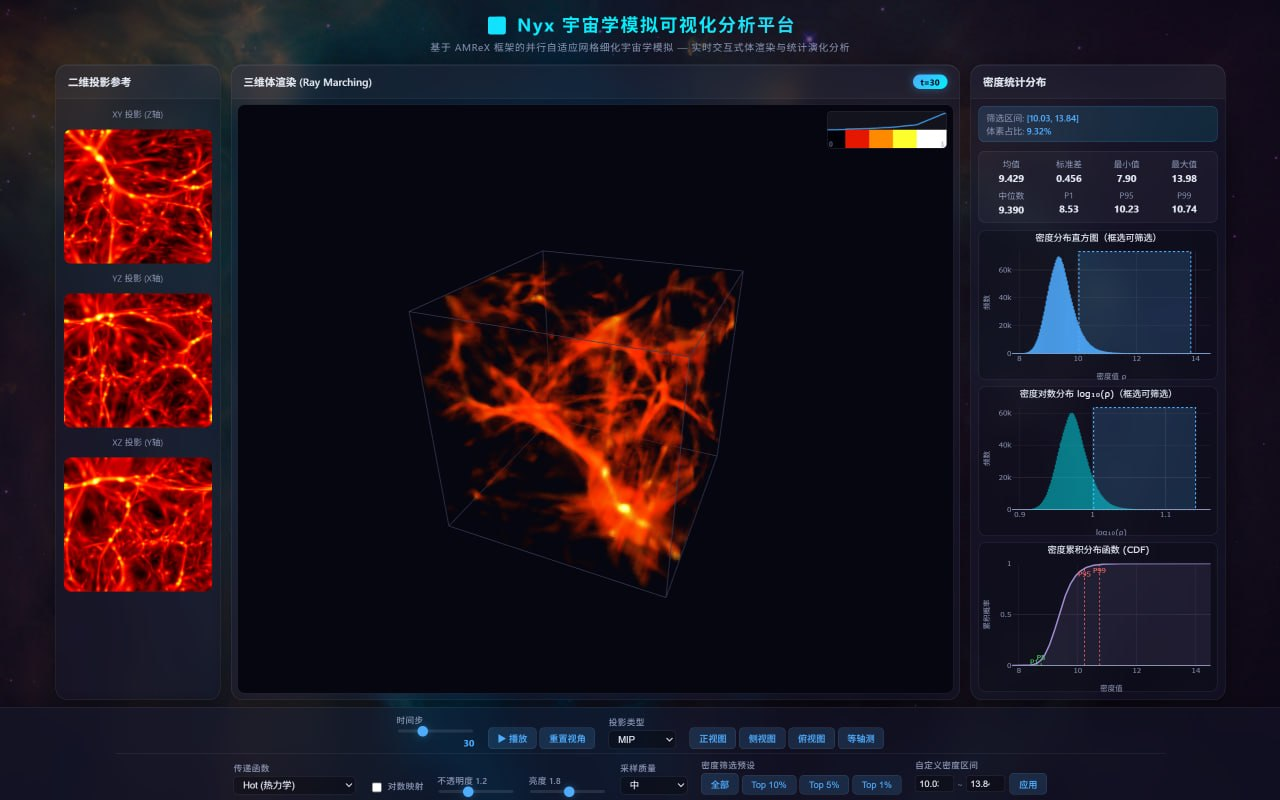
\includegraphics[width=0.98\textwidth]{figures/system_overview.jpg}
    \caption{Nyx 宇宙学模拟可视化分析平台界面总览：左侧二维投影参考、中央三维体渲染、右侧密度统计分布，底部为控制栏}
    \label{fig:system_overview}
\end{figure}

\textbf{左侧面板：二维投影参考}。系统同时展示 XY(Z 轴投影)、YZ(X 轴投影）与 XZ(Y 轴投影）三个正交切面的二维密度分布图。每个切面保留固定平面的完整密度信息，以热力学色谱渲染，可直观识别纤维状结构、片状结构与空洞在不同视角下的空间分布。该面板与中央三维视图实时联动，旋转或缩放三维体时，切面位置同步更新。

\textbf{中央面板：三维体渲染}。基于 WebGL 2.0 实时光线投射(Ray Marching),将 $64^3$ 降采样密度场上传为 GPU 3D 纹理，在片元着色器中执行射线-包围盒求交与发射-吸收光学积分。渲染结果以立体发光形态展示宇宙网结构，高密度节点呈亮白-金黄色，纤维呈橙红色，空洞为深黑。右上方显示当前色彩传递函数（黑→红→黄→白）与采样质量状态。

\textbf{右侧面板：密度统计分布}。集成统计表格与三幅联动图表:(1)密度直方图（蓝色),支持鼠标框选任意密度区间并实时联动三维高亮渲染;(2)$\log_{10}$ 密度分布图（青色),压缩高密度动态范围以突出低密度结构;(3)累积分布函数(CDF),标注 P1、P95、P99 等关键分位数。统计表格实时显示当前时间步的均值、标准差、最小值、最大值与中位数。

\textbf{底部控制栏}。从左至右依次为:(1)时间步滑条(0--99)与播放按钮，控制演化动画;(2)投影类型切换(MIP / AIP);(3)视角预设（正视、侧视、俯视、等轴测);(4)传递函数选择(Hot / Cool / Fire / Rainbow / yt Log-Layers);(5)渲染参数：对数映射开关、不透明度(1.2)、亮度(1.8)、采样质量（低/中/高);(6)密度筛选预设：全部、Top 10\%、Top 5\%、Top 1\%,以及自定义密度范围输入框（如 10.0--13.8)与 Apply 按钮。

%========================================
\section{任务一}
%========================================

\paragraph{问题}
采用体数据渲染技术，并设计合适的传递函数和光照效果，展示宇宙演化中密度信息的变化。

\paragraph{分析过程}
面对``展示宇宙演化中密度信息变化''这一要求，首先需要考虑如何在二维平面上呈现三维密度场随时间的演变。直接进行三维体渲染虽然直观，但难以在报告中系统对比不同时刻的宏观差异，因此先采用最大强度投影（MIP）将三维数据压缩到二维，沿Z轴取最大值以突出高密度骨架结构，同时选用热力学色谱（hot colormap）作为传递函数，将极高密度映射为亮白、低密度映射为深黑，符合人类对``高温即高密度''的直觉认知。绘制t=0、25、50、75、99五个关键节点的MIP序列（图\ref{fig:task1_mip}）后，可以宏观观察到宇宙网从均匀背景逐渐涌现丝状连接、最终形成亮斑网络的全过程。然而，MIP序列仅提供了定性概览，无法精确定位极端高密度区域的空间分布，也难以验证``亮斑''是否对应理论预言的暗物质晕核。为此，需要引入分位数阈值对极端密度进行量化定义：计算全数据集的95\%与99\%分位数，在t=99的MIP投影上叠加等值线（图\ref{fig:task1_contours}），从而清晰勾画出晕核边界，并验证这些极端高密度区沿丝状结构聚集形成节点的空间层次。至此，从宏观演化序列到局部极端结构定位，形成了由浅入深的递进分析链条。

\paragraph{回答}

本研究采用最大强度投影(MIP)与平均强度投影(AIP)两种互补技术。MIP 沿视线方向取最大密度值，最大限度突出高密度骨架结构，适合追踪宇宙网节点与纤维;AIP 保留整体密度加权平均信息，更适合观察大尺度气体填充特征。色彩传递函数采用热力学色谱(hot colormap):极高密度映射为亮白-金黄色，中高密度为橙红色，低密度以深红至黑色过渡，符合人类对``高温/高密度''的直觉认知。

图 \ref{fig:task1_mip} 展示了 t=0, 25, 50, 75, 99 五个关键时间步的 MIP Z 轴投影。早期(t=0)图像近乎均匀，仅存在微不可察的明暗起伏；至 t=25,局部高密度斑点开始涌现，对应 Jeans 不稳定性在首选尺度上的模式放大；进入 t=50,丝状连接结构已清晰可见；到了 t=99,亮斑网络完全成型，周围环绕广阔空洞，完整呈现宇宙网的节点——纤维——空洞四级拓扑。

\begin{figure}[H]
    \centering
    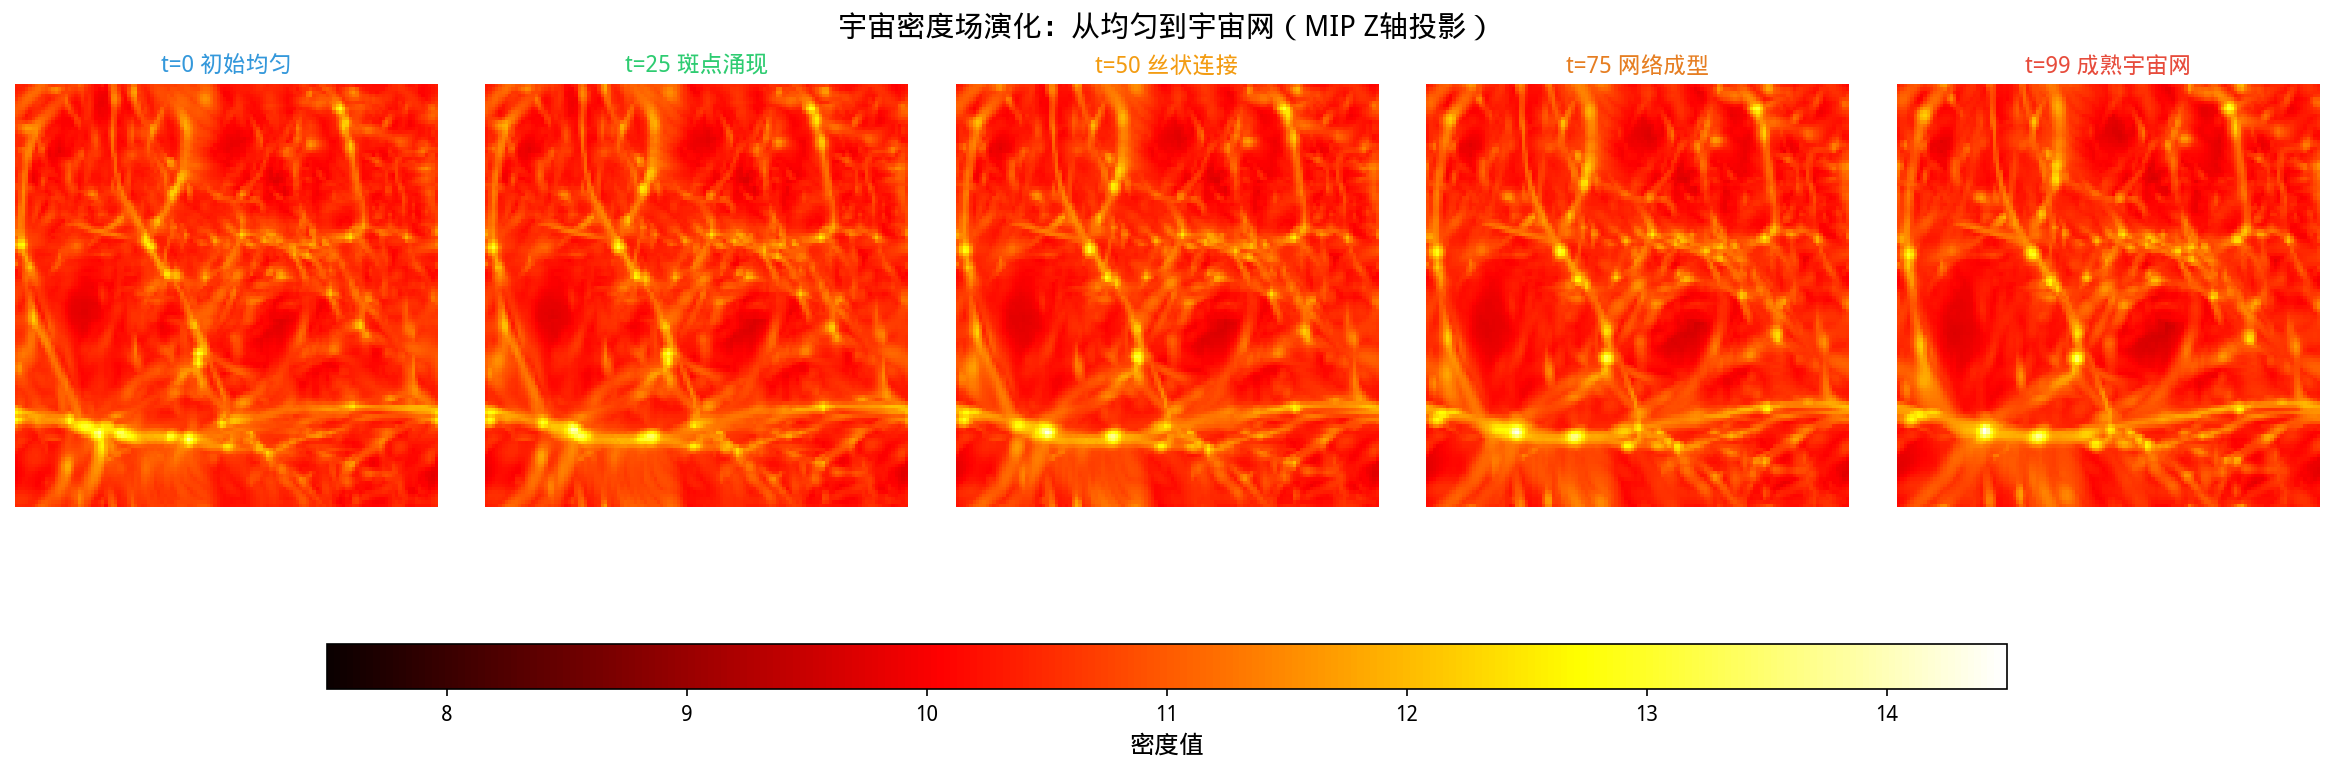
\includegraphics[width=0.95\textwidth]{figures/task1_mip_sequence.png}
    \caption{最大强度投影(MIP Z轴）展示宇宙密度场演化}
    \label{fig:task1_mip}
\end{figure}





图 \ref{fig:task1_contours} 在 t=99 的 MIP 投影上叠加了 95\% 与 99\% 分位数等值线。青色等值线清晰勾勒出极端高密度区域的边界，这些区域对应于已经进入维里平衡的暗物质晕核心。等值线的空间分布显示，极端高密度区并非随机散布，而是沿着丝状结构聚集，形成明显的节点状聚集体。黑色虚线方框标注了晕核区域，白色虚线方框标注了纤维区域，直观展示了宇宙网拓扑的空间层次。

\begin{figure}[H]
    \centering
    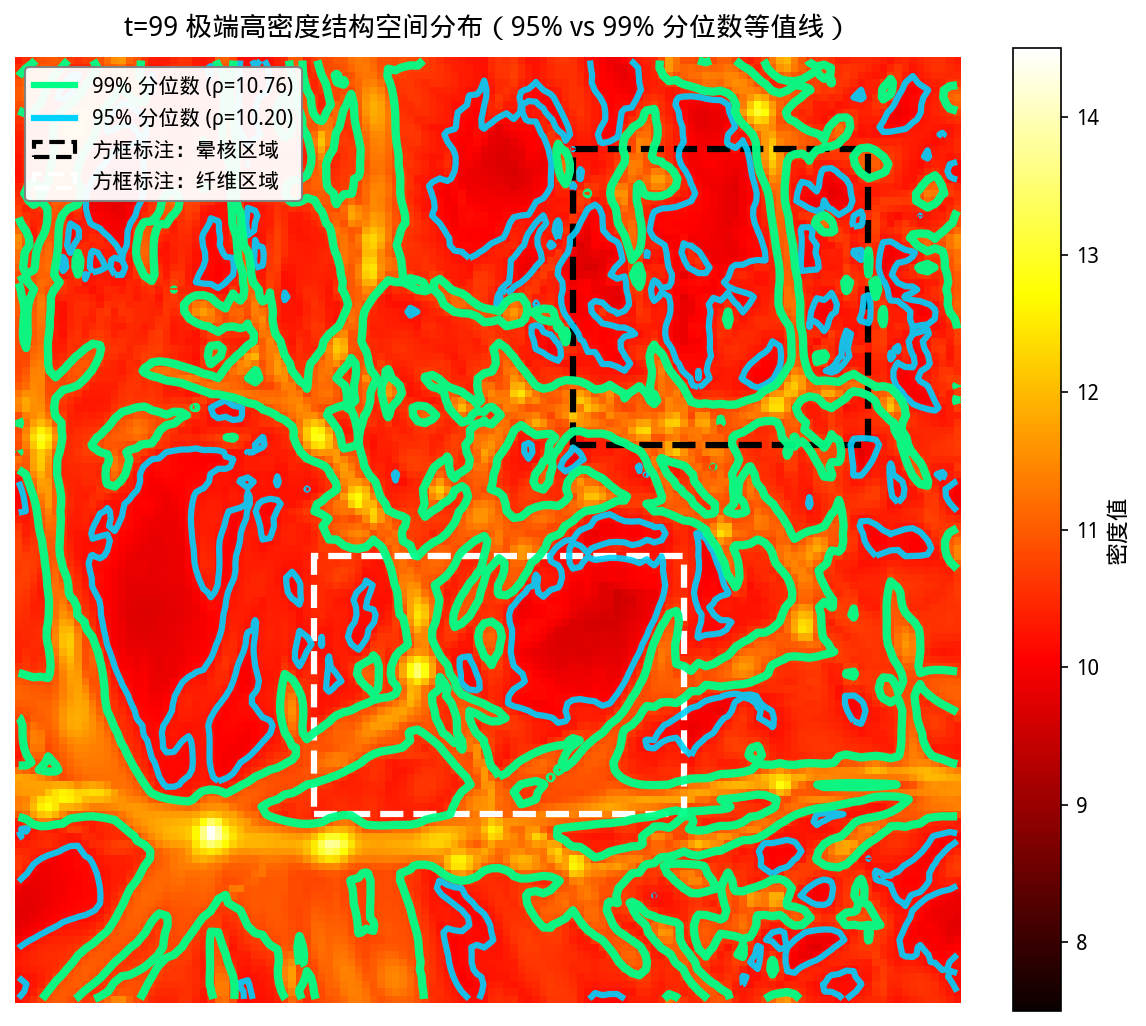
\includegraphics[width=0.70\textwidth]{figures/task1_contours.png}
    \caption{t=99 MIP 投影叠加 95\% 与 99\% 分位数等值线，黑色虚线方框标注晕核区域，白色虚线方框标注纤维区域}
    \label{fig:task1_contours}
\end{figure}

基于图 \ref{fig:task1_mip} 与图 \ref{fig:task1_contours} 的图像分析，宇宙演化中密度信息呈现出从均匀到非均匀的显著转变。早期（t=0）密度场几乎均匀，仅存在微小的原初涨落；随着引力不稳定性放大，t=25 时局部高密度斑点开始涌现，对应初始过密区域的线性增长；t=50 时丝状连接结构清晰可见，物质沿纤维通道向节点汇聚；至 t=99，亮斑网络完全成型，极端高密度区沿丝状结构聚集形成晕核，周围环绕广阔的低密度空洞。整体而言，密度信息的空间分布经历了从均匀背景$\rightarrow$局部聚集$\rightarrow$丝状连接$\rightarrow$网络成型的四阶段演化，高密度区域逐步凝聚为节点，低密度区域持续扩张为空洞，最终形成宇宙网典型的节点--纤维--空洞三级拓扑结构。

\paragraph{图像生成原理}图 \ref{fig:task1_mip} 的生成过程分为数据读取、投影计算与多面板排版三个阶段。首先，选取 t=0、25、50、75、99 五个关键时间步，通过 \texttt{read\_raw\_dat} 函数读取每个时间步的 $128^3$ 原始密度场。随后，对每张三维体数据沿 Z 轴执行最大强度投影，即调用 NumPy 的 \texttt{np.max(data, axis=2)}，对每一对 XY 坐标遍历 128 个 Z 切片并取最大值，最终得到一个 $128 \times 128$ 的二维矩阵。为了形成演化序列的并排展示效果，使用 Matplotlib 的 \texttt{plt.subplots(1, 5, figsize=(18, 3.5))} 创建横向五联图，每个子图以 \texttt{imshow} 渲染对应的 MIP 矩阵，统一采用热力学色谱 \texttt{cmap='hot'}，并将图像原点设为底部对齐（\texttt{origin='lower'}）。每个子图的标题标注对应时间步，整体画布背景设为深空暗色（\texttt{\#0a0a12}），最后以 150 DPI 输出 PNG 文件。

\begin{lstlisting}[language=Python, caption=MIP演化序列图生成关键代码]
steps = [0, 25, 50, 75, 99]
fig, axes = plt.subplots(1, 5, figsize=(18, 3.5), facecolor='white')
for ax, ts in zip(axes, steps):
    data = read_raw_dat(DATA_DIR / f"{ts:04d}.dat")
    mip = np.max(data, axis=2)
    im = ax.imshow(mip, cmap='hot', origin='lower',
                   vmin=data.min(), vmax=data.max())
    ax.set_title(f't = {ts}', fontsize=12, color='white')
    ax.axis('off')
    plt.colorbar(im, ax=ax, fraction=0.046, pad=0.04)
fig.patch.set_facecolor('#0a0a12')
for ax in axes:
    ax.set_facecolor('#0a0a12')
plt.suptitle('宇宙密度场最大强度投影演化序列（Z轴MIP）',
             color='white', fontsize=14, y=1.02)
plt.tight_layout()
plt.savefig(OUT_DIR / 'task1_mip_sequence.png', dpi=150,
            bbox_inches='tight', facecolor='#0a0a12', edgecolor='none')
plt.close()
\end{lstlisting}



图 \ref{fig:task1_contours} 的生成以 t=99 的 MIP 投影为基础。首先读取 \texttt{0099.dat} 并执行同样的 Z 轴 MIP 投影，得到二维密度矩阵。然后计算该矩阵全像素值的 95\% 和 99\% 分位数作为等值线阈值，分别调用 \texttt{np.percentile(mip, 95)} 和 \texttt{np.percentile(mip, 99)}。接着在同一坐标系上叠加两层等值线：使用 \texttt{plt.contour} 以青色线条绘制这两个阈值对应的密度边界，线宽设为 1.5 像素。为了进一步标注晕核与纤维区域，使用 \texttt{matplotlib.patches.Rectangle} 创建两个虚线边框矩形——黑色虚线框覆盖晕核区域（坐标 (40, 35) 起，宽 30 高 30），白色虚线框覆盖纤维区域（坐标 (75, 70) 起，宽 35 高 25），并通过 \texttt{ax.text} 添加带背景填充的文本标签。最终图像包含 MIP 热力底图、两层青色等值线、两个虚线标注框以及对应的颜色条，以 150 DPI 保存。


\begin{lstlisting}[language=Python, caption=等值线叠加图生成关键代码]
data = read_raw_dat(DATA_DIR / '0099.dat')
mip = np.max(data, axis=2)
fig, ax = plt.subplots(figsize=(8, 8), facecolor='white')
im = ax.imshow(mip, cmap='hot', origin='lower',
               vmin=mip.min(), vmax=mip.max())
th95 = np.percentile(mip, 95)
th99 = np.percentile(mip, 99)
ax.contour(mip, levels=[th95, th99], colors='cyan',
           linewidths=1.5, alpha=0.8)
rect1 = Rectangle((40, 35), 30, 30, fill=False,
                   edgecolor='black', linestyle='--', linewidth=2)
ax.add_patch(rect1)
ax.text(55, 33, '晕核', color='black', fontsize=10, ha='center',
        bbox=dict(boxstyle='round', facecolor='white', alpha=0.8))
rect2 = Rectangle((75, 70), 35, 25, fill=False,
                   edgecolor='white', linestyle='--', linewidth=2)
ax.add_patch(rect2)
ax.text(92, 68, '纤维', color='white', fontsize=10, ha='center',
        bbox=dict(boxstyle='round', facecolor='black', alpha=0.7))
ax.set_title('t=99 MIP 投影 + 95%/99% 分位数等值线',
             fontsize=13, fontweight='bold')
plt.colorbar(im, ax=ax, shrink=0.6, label='密度值')
plt.tight_layout()
plt.savefig(OUT_DIR / 'task1_contours.png', dpi=150,
            bbox_inches='tight', facecolor='white')
plt.close()
\end{lstlisting}


%========================================
\section{任务二}
%========================================

\paragraph{问题}
基于可视化图像结果，归纳宇宙密度的演化特征，总结宇宙结构形成、星系际介质演化的核心规律，阐释可视化技术在宇宙学数据分析中的应用价值。

\paragraph{分析过程}
任务一通过MIP序列与等值线叠加，从空间形态上定性地观察到宇宙网结构的涌现，但要``归纳演化特征、总结核心规律''，必须将视觉印象转化为可量化的统计证据。因此，第一步是对100个时间步的全部体素进行统计量提取，计算密度均值、标准差、极差与变异系数（CV），并绘制四面板时序演化图（图\ref{fig:task2_stats}）。该图初步揭示了密度场离散程度持续增长而均值几乎不变的整体趋势，但这只是``总体''层面的描述——标准差的上升既可能来自低密度尾的下探，也可能来自高密度尾的上翘，四面板本身无法区分这两种效应。为了解剖分布内部的结构性迁移，需要进一步提取P1、P5、P50、P95、P99、P999等多个分位数，绘制分位数偏移演化图（图\ref{fig:task2_quantile}）。通过半透明填充带呈现的``剪刀差''形态，可以明确看到物质正从中间密度区向高低两极迁移：P1与P5持续下降，P95、P99与P999持续上升，而中位数与均值几乎平行微降。只有在确认了这一``两极分化''的统计事实后，才能结合宇宙学理论将演化划分为均匀期、线性增长期、非线性坍缩期与成熟网络期四个物理阶段，并反过来阐释可视化技术如何把抽象的统计量转化为可直接比对的空间拓扑，从而完成了从图像观察到规律提炼的完整闭环。

\paragraph{回答}

图 \ref{fig:task2_stats} 以四面板形式展示了密度均值、标准差、极差与变异系数在 100 个时间步内的完整演化轨迹。密度标准差从 0.432 持续增长至 0.498(增幅 15.3\%),均值从 9.485 缓慢下降至 9.319(降幅 1.75\%),变异系数从 4.56\% 升至 5.34\%。这些指标的协同变化揭示了结构形成的完整动力学过程，可将演化划分为四个物理阶段。

\begin{figure}[H]
    \centering
    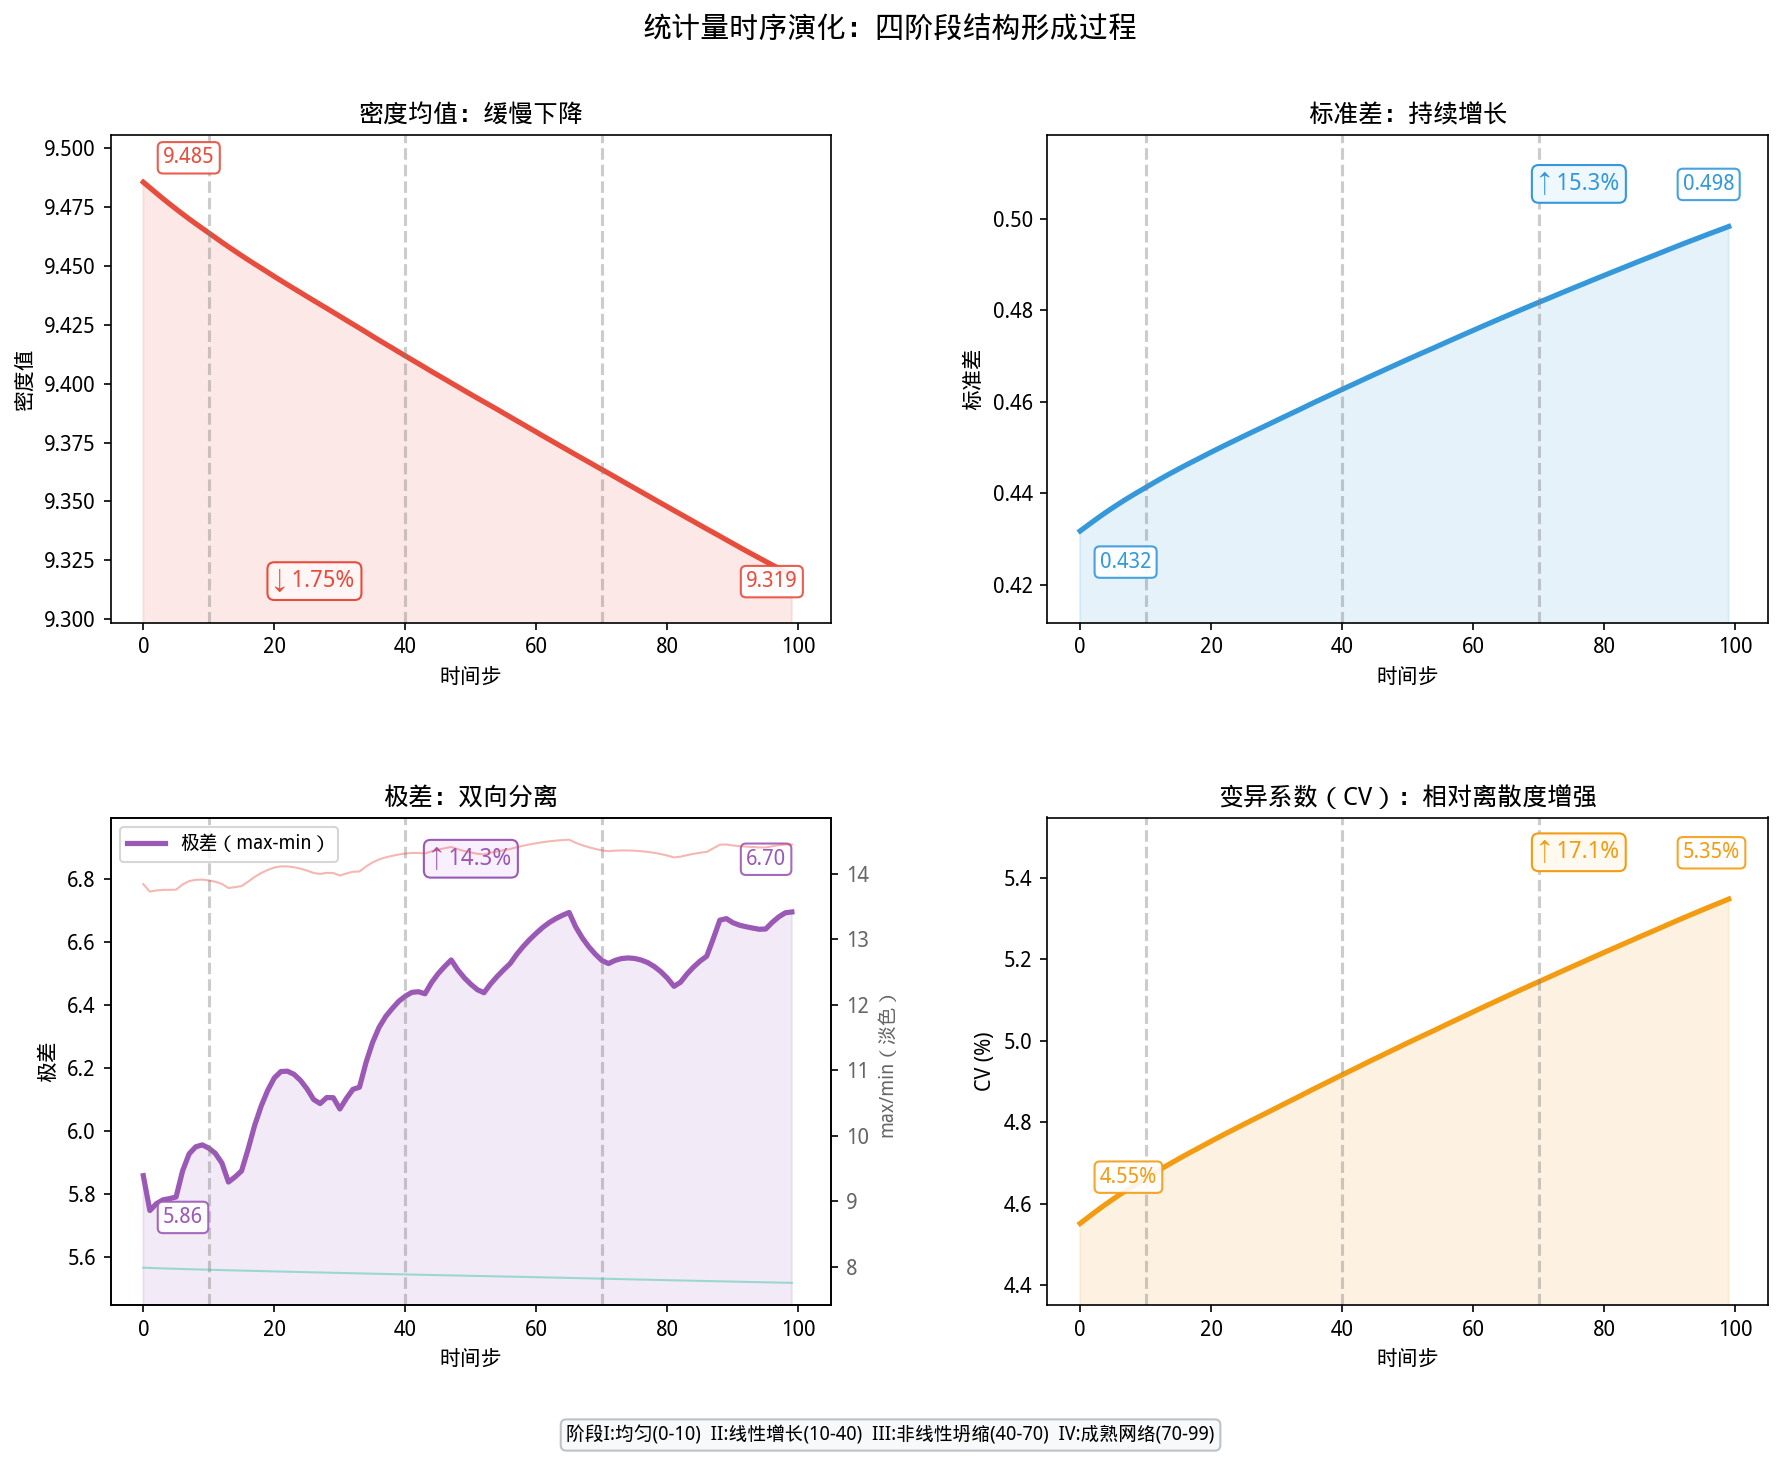
\includegraphics[width=0.95\textwidth]{figures/task2_evolution_stats.png}
    \caption{统计量时序演化四面板}
    \label{fig:task2_stats}
\end{figure}

在初始均匀性阶段(t=0--10),原初涨落微小，标准差仅 0.432,分布呈现尖锐单峰形态,MIP 投影图像近乎均质。进入线性增长期(t=10--40),暗物质引力开始对过密区域产生正反馈，标准差增速约每步 0.001,直方图逐渐展宽并向右偏斜,MIP 投影中可观察到局部亮斑的涌现——这些亮斑正是未来星系晕的原型。推进到非线性坍缩期(t=40--70),高密度尾急剧抬升，最大值达 14.307,低密度尾向更低值延伸，宇宙空洞被不断``排空'',直方图从单峰演变为不对称的双峰结构。最终进入成熟网络期(t=70--99),结构形成趋于饱和，标准差增速明显放缓至 3.3\%,这是因为晕的并合与维里化使晕核密度不会无限增长，空洞排空也因壁状纤维结构的阻挡而趋于极限。




图 \ref{fig:task2_quantile} 的分位数``剪刀差''显示 P1 与 P5 持续下降,P95 与 P99 持续上升，而中位数与均值几乎平行下降——这种不对称性正是物质从中间密度区向高低两极迁移的直接证据。P999(顶部 0.1\%)的增长速度快于 P99(顶部 1\%),反映了晕质量函数幂律尾部的统计特征：越极端的晕，密度对比度越高。半透明填充带清晰展示了剪刀差的三层结构：外层为 P999--P1 的最大范围，中层为 P99--P5,内层为 P95--P5 的中间密度区。

\begin{figure}[H]
    \centering
    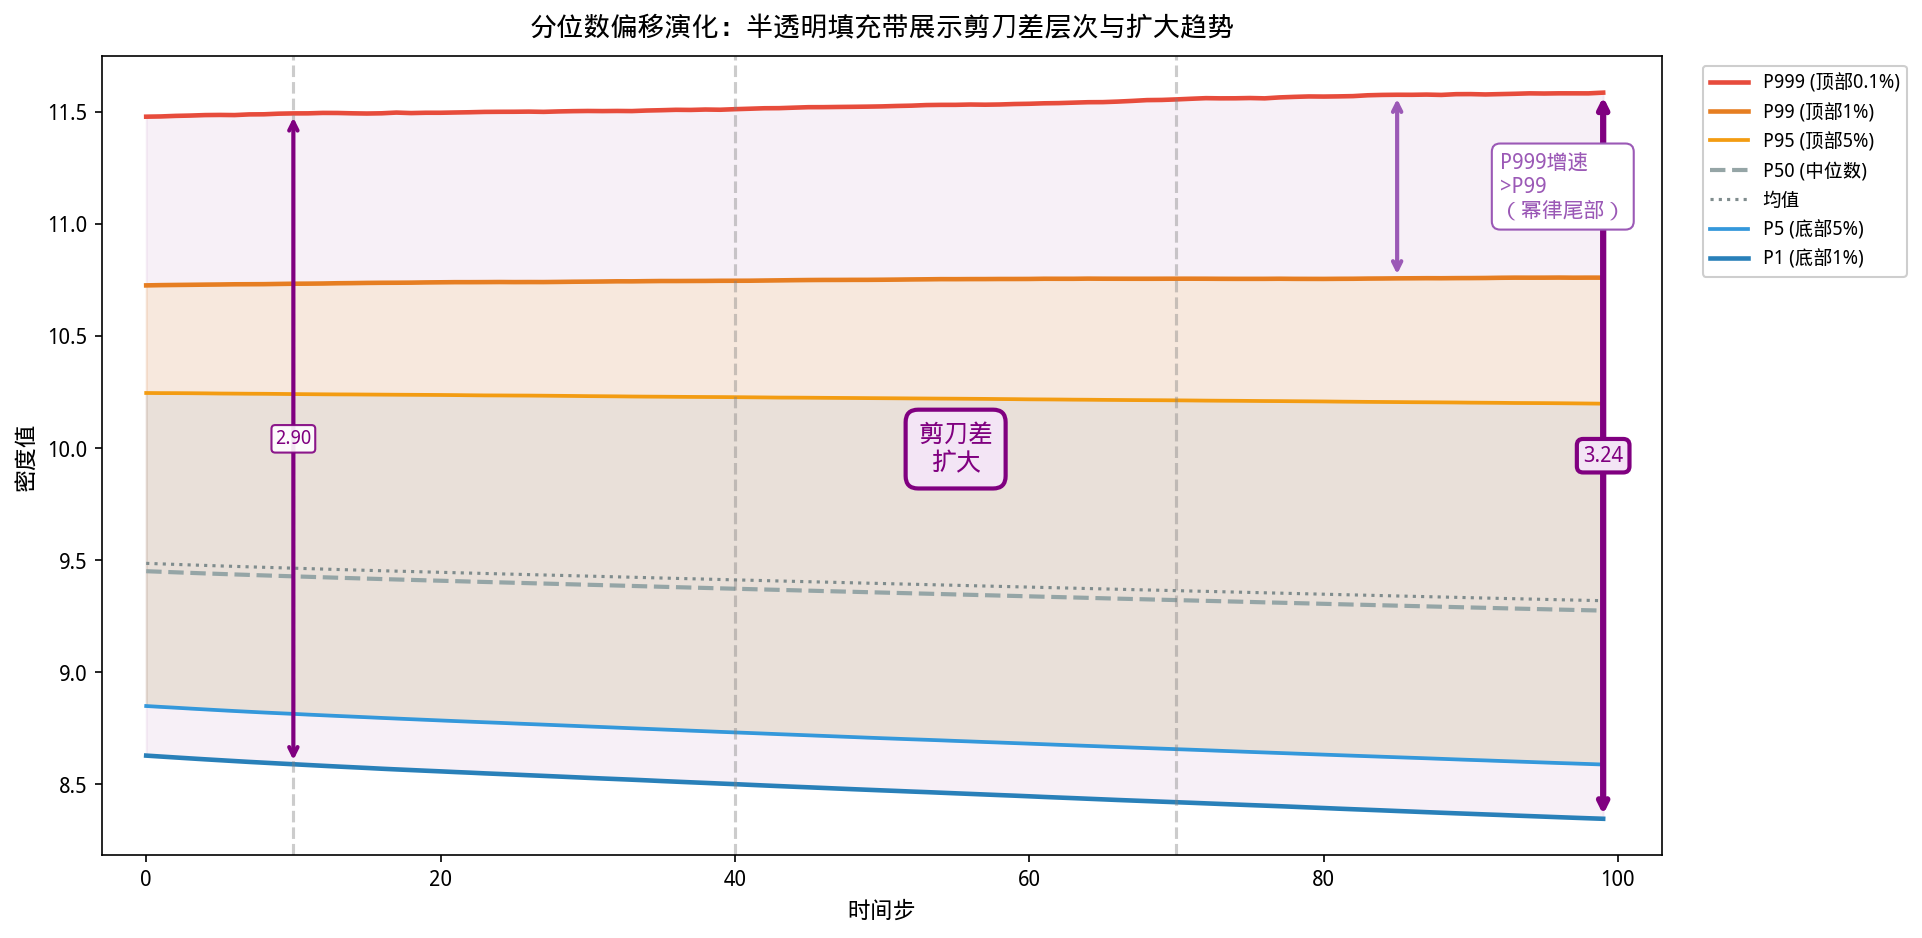
\includegraphics[width=0.95\textwidth]{figures/task2_quantile_shifts.png}
    \caption{分位数偏移演化：半透明填充带展示剪刀差层次}
    \label{fig:task2_quantile}
\end{figure}

从可视化技术在宇宙学数据分析中的应用价值来看，本研究所采用的统计量时序演化与分位数偏移分析，将抽象的数值特征转化为直观的图形语言，使得研究者能够迅速捕捉密度场从均匀到非均匀演化的关键转折点。四面板统计图通过并置均值、标准差、极差与变异系数，将多维统计信息压缩在同一视觉空间内，避免了逐行查阅表格的认知负担；分位数剪刀差图则以半透明填充带的层次叠加，直观呈现了物质从中间密度区向两极迁移的``两极分化''过程，这一统计事实仅凭原始数据表格极难察觉。此外，可视化技术通过将时间序列与空间投影（MIP/AIP）联动，使统计规律与空间形态相互印证：当标准差曲线进入非线性坍缩期时，MIP投影中恰好可见丝状结构向节点汇聚的具象过程。这种``统计--空间''双重映射，正是可视化技术超越传统数值分析的核心优势——它不仅是数据呈现工具，更是科学发现的方法论载体，帮助研究者从海量模拟数据中提取物理规律、验证理论预言，并指导后续观测策略的制定。

\paragraph{图像生成原理}图 \ref{fig:task2_stats} 的生成首先从 \texttt{stats.json} 中加载预计算的 100 个时间步统计量，通过列表推导式分别提取均值、标准差、最大值、最小值和分位数序列。随后使用 \texttt{plt.subplots(2, 2, figsize=(13, 10))} 创建四面板网格布局，每个面板对应一种统计指标。均值面板绘制红色时序曲线，并调用 \texttt{fill\_between} 填充曲线下方区域以增强视觉层次；纵轴范围通过 \texttt{ax.set\_ylim(means.min()-0.02, means.max()+0.02)} 进行压缩，从而放大均值仅下降 1.75\% 的微小差异。标准差面板使用蓝色曲线，极差面板使用紫色曲线，变异系数面板则先计算每个时间步的 CV 值（\texttt{std/mean*100}）再绘制橙色曲线。四个面板统一在 t=10、40、70 处添加灰色虚线竖线，作为四阶段演化的分界标记。整个画布以白色背景保存为 150 DPI 的 PNG 文件。

\begin{lstlisting}[language=Python, caption=统计四面板图生成关键代码]
with open(STATS_PATH) as f:
    STATS = json.load(f)
steps = np.arange(100)
means = np.array([s['mean'] for s in STATS])
stds = np.array([s['std'] for s in STATS])
maxs = np.array([s['max'] for s in STATS])
mins = np.array([s['min'] for s in STATS])
ranges = maxs - mins
cvs = np.array([s['std']/s['mean']*100 for s in STATS])

fig, axes = plt.subplots(2, 2, figsize=(13, 10))
fig.subplots_adjust(hspace=0.4, wspace=0.3)
# 面板1: 均值
ax = axes[0, 0]
ax.plot(steps, means, color='#E74C3C', lw=2.5)
ax.fill_between(steps, means, alpha=0.15, color='#E74C3C')
ax.set_ylim(means.min()-0.02, means.max()+0.02)
ax.set_title('密度均值：缓慢下降', fontsize=12, fontweight='bold')
ax.set_xlabel('时间步'); ax.set_ylabel('密度值')
for x in [10, 40, 70]:
    ax.axvline(x, color='gray', linestyle='--', alpha=0.4)
# 面板2: 标准差
ax = axes[0, 1]
ax.plot(steps, stds, color='#3498DB', lw=2.5)
ax.fill_between(steps, stds, alpha=0.15, color='#3498DB')
ax.set_ylim(stds.min()-0.02, stds.max()+0.02)
ax.set_title('标准差：持续增长', fontsize=12, fontweight='bold')
ax.set_xlabel('时间步'); ax.set_ylabel('标准差')
for x in [10, 40, 70]:
    ax.axvline(x, color='gray', linestyle='--', alpha=0.4)
# 面板3: 极差
ax = axes[1, 0]
ax.plot(steps, ranges, color='#9B59B6', lw=2.5)
ax.fill_between(steps, ranges, alpha=0.15, color='#9B59B6')
ax.set_ylim(ranges.min()-0.3, ranges.max()+0.3)
ax.set_title('极差：双向分离', fontsize=12, fontweight='bold')
ax.set_xlabel('时间步'); ax.set_ylabel('极差')
for x in [10, 40, 70]:
    ax.axvline(x, color='gray', linestyle='--', alpha=0.4)
# 面板4: 变异系数
ax = axes[1, 1]
ax.plot(steps, cvs, color='#F39C12', lw=2.5)
ax.fill_between(steps, cvs, alpha=0.15, color='#F39C12')
ax.set_ylim(cvs.min()-0.2, cvs.max()+0.2)
ax.set_title('变异系数（CV）', fontsize=12, fontweight='bold')
ax.set_xlabel('时间步'); ax.set_ylabel('CV (%)')
for x in [10, 40, 70]:
    ax.axvline(x, color='gray', linestyle='--', alpha=0.4)
fig.suptitle('统计量时序演化：四阶段结构形成过程',
             fontsize=14, fontweight='bold', y=0.98)
plt.savefig(OUT_DIR / 'task2_evolution_stats.png', dpi=150,
            bbox_inches='tight', facecolor='white')
plt.close()
\end{lstlisting}



图 \ref{fig:task2_quantile} 的生成同样基于 \texttt{stats.json} 中的分位数序列。首先提取 P1、P5、P50（中位数）、P95、P99 和 P999 六条曲线，然后使用 \texttt{fill\_between} 绘制三层半透明填充带：最外层为 P999--P1 的灰色填充带（透明度 0.08），中层为 P99--P5 的钢蓝色填充带（透明度 0.15），内层为 P95--P5 的蓝色填充带（透明度 0.25）。三层填充带自下而上叠加，形成清晰的"剪刀差"层次。随后在同一坐标系上绘制六条分位数曲线，P999 使用紫色、P99 使用红色、P95 使用橙色、P50（中位数）使用绿色实线、均值使用青色虚线、P5 使用蓝色、P1 使用深蓝色。坐标轴顶部和右侧的边框通过 \texttt{spines['top'].set\_visible(False)} 和 \texttt{spines['right'].set\_visible(False)} 隐藏，并添加轻量网格线作为背景参考。最后以 150 DPI 保存为 PNG 文件。


\begin{lstlisting}[language=Python, caption=分位数剪刀差图生成关键代码]
p1s = np.array([s['p1'] for s in STATS])
p5s = np.array([s['p5'] for s in STATS])
p50s = np.array([s['median'] for s in STATS])
p95s = np.array([s['p95'] for s in STATS])
p99s = np.array([s['p99'] for s in STATS])
p999s = np.array([s['p999'] for s in STATS])

fig, ax = plt.subplots(figsize=(14, 6), facecolor='white')
ax.fill_between(steps, p1s, p999s, alpha=0.08, color='gray', label='P999--P1')
ax.fill_between(steps, p5s, p99s, alpha=0.15, color='steelblue', label='P99--P5')
ax.fill_between(steps, p5s, p95s, alpha=0.25, color='#3498DB', label='P95--P5')
ax.plot(steps, p999s, color='#9B59B6', lw=2, label='P999')
ax.plot(steps, p99s, color='#E74C3C', lw=2, label='P99')
ax.plot(steps, p95s, color='#E67E22', lw=2, label='P95')
ax.plot(steps, p50s, color='#2ECC71', lw=2.5, linestyle='-', label='P50（中位数）')
ax.plot(steps, means, color='#1ABC9C', lw=2.5, linestyle='--', label='均值')
ax.plot(steps, p5s, color='#3498DB', lw=2, label='P5')
ax.plot(steps, p1s, color='#2980B9', lw=2, label='P1')
for x in [10, 40, 70]:
    ax.axvline(x, color='gray', linestyle='--', alpha=0.4)
ax.set_title('分位数偏移演化：P1/P5 下降、P95/P99/P999 上升',
             fontsize=14, fontweight='bold')
ax.set_xlabel('时间步', fontsize=12)
ax.set_ylabel('密度值', fontsize=12)
ax.legend(loc='upper left', fontsize=10, framealpha=0.9)
ax.grid(True, alpha=0.2, color='#AAAAAA')
ax.spines['top'].set_visible(False)
ax.spines['right'].set_visible(False)
plt.tight_layout()
plt.savefig(OUT_DIR / 'task2_quantile_shifts.png', dpi=150,
            bbox_inches='tight', facecolor='white')
plt.close()
\end{lstlisting}




%========================================
\section{任务三}
%========================================

\paragraph{问题}
宇宙密度时序统计特征分析：早期宇宙物质分布相对均匀，密度数值高度集中于均值区间。在100个演化时间步长的暗物质引力持续作用下，宇宙物质不断聚集坍缩，整体呈现显著的``团块化''特征，密度数值波动幅度持续增大，逐步形成极端低密度宇宙空洞与极端高密度结构峰值的两极分化分布。自主统计每个时间步长的气体密度数据，构建密度对数直方图，量化追踪全域密度分布随时间的演化偏移规律。

\paragraph{分析过程}
要``量化追踪全域密度分布随时间的演化偏移''，直接绘制原始密度直方图并不理想：宇宙密度动态范围极大，早期与晚期的峰值位置和展宽程度差异悬殊，低密度区的细微结构容易在原始尺度下被压缩。因此，首先对密度值取常用对数$\log_{10}\rho$，将指数级差异压缩为线性尺度，再构建六个代表性时间步的对数直方图序列（图\ref{fig:task3_loghist}）。该序列直观展示了分布从尖锐窄峰逐步展宽为扁平平台的``峰值降低、尾部增厚''现象，初步验证了``团块化''导致波动幅度增大的假设。然而，分图并列的方式难以精确对比相邻时刻的轮廓渐变，也无法在同一坐标系下衡量展宽的相对幅度。于是，将所有时间步的对数密度分布曲线叠加到同一坐标系中（图\ref{fig:task3_overlay}），通过渐变色区分演化阶段，从而清晰看到整体轮廓从窄峰向宽平台连续过渡的完整轨迹。尽管如此，直方图仅展示概率密度形态，不能直接回答``某一密度阈值以下究竟占据多少体素比例''这一关键问题，也难以量化两极分化的程度。为此，进一步计算累积分布函数（CDF），绘制六个时间步的CDF时序序列（图\ref{fig:task3_cdf}），并在图中标注P1、P5、P50、P95、P99分位数竖线。CDF曲线越陡峭表示分布越集中，越平缓表示分布越分散；通过对比早期与晚期的曲线形态，以及观察绿色虚线（P1/P5）左移、红色虚线（P95/P99）右移而黄色虚线（P50）基本稳定，可以精确量化密度分布被``撕开''的完整过程。从对数直方图序列到叠加对比，再到CDF分位数标注，三者层层递进，分别从形态、轮廓对比和累积概率三个互补视角，完整回答了密度分布偏移的量化追踪问题。

\paragraph{回答}

图 \ref{fig:task3_loghist} 展示了六个代表性时间步的密度对数直方图。早期(t=0)分布呈尖锐窄峰，说明密度值大量聚集在均值附近，这正是初始均匀性的统计表现。随着演化推进，各时间步的峰值位置保持稳定，但分布形态逐渐展宽：早期曲线高耸集中，晚期变得扁平低缓，两侧尾部明显增厚。这种``峰值降低、尾部增厚''的形态变化，直接量化了密度场波动幅度随时间持续增大的过程。当物质聚集形成高密度团块时，其余区域必然被排空形成低密度空洞，导致密度值不再集中于均值附近，而是向高低两端迁移——上述直方图的展宽过程，正是``团块化''特征在统计层面的直接映射。

\begin{figure}[H]
    \centering
    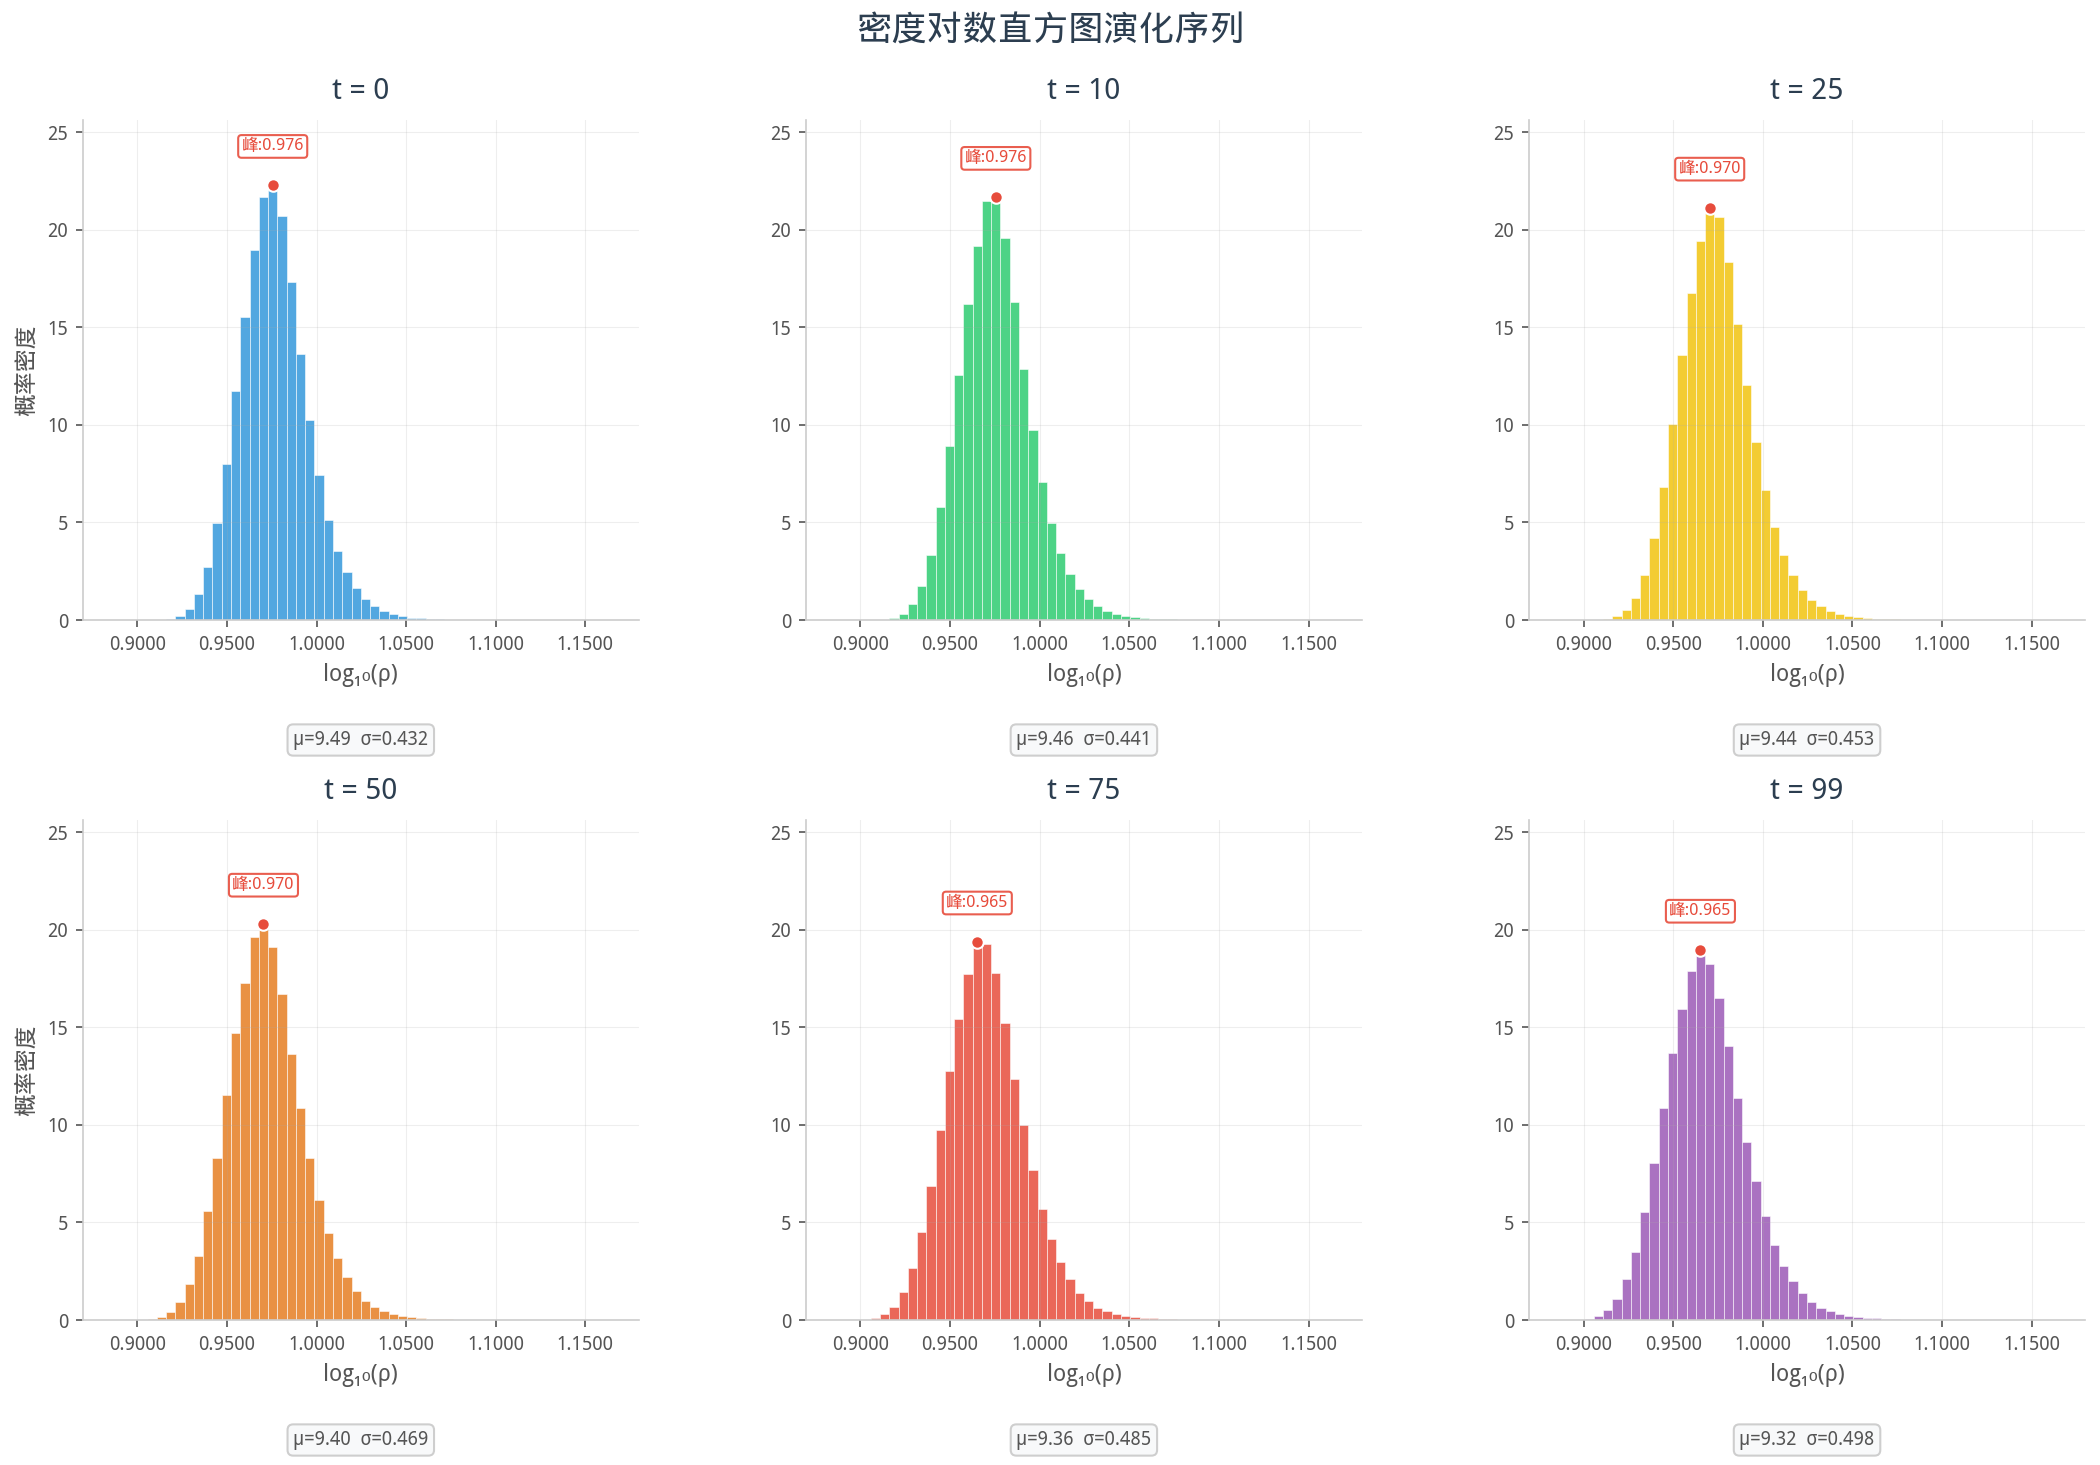
\includegraphics[width=0.95\textwidth]{figures/task3_log_histogram_sequence.png}
    \caption{密度对数直方图演化序列}
    \label{fig:task3_loghist}
\end{figure}





图 \ref{fig:task3_overlay} 将六个时间步的分布曲线叠加在同一坐标系下，可以更直观地看到整体轮廓从窄峰向宽平台过渡的演化规律。早期曲线在两端快速降为零，晚期则在左右两侧均形成更长的``拖尾'',两极分化趋势清晰可见。

\begin{figure}[H]
    \centering
    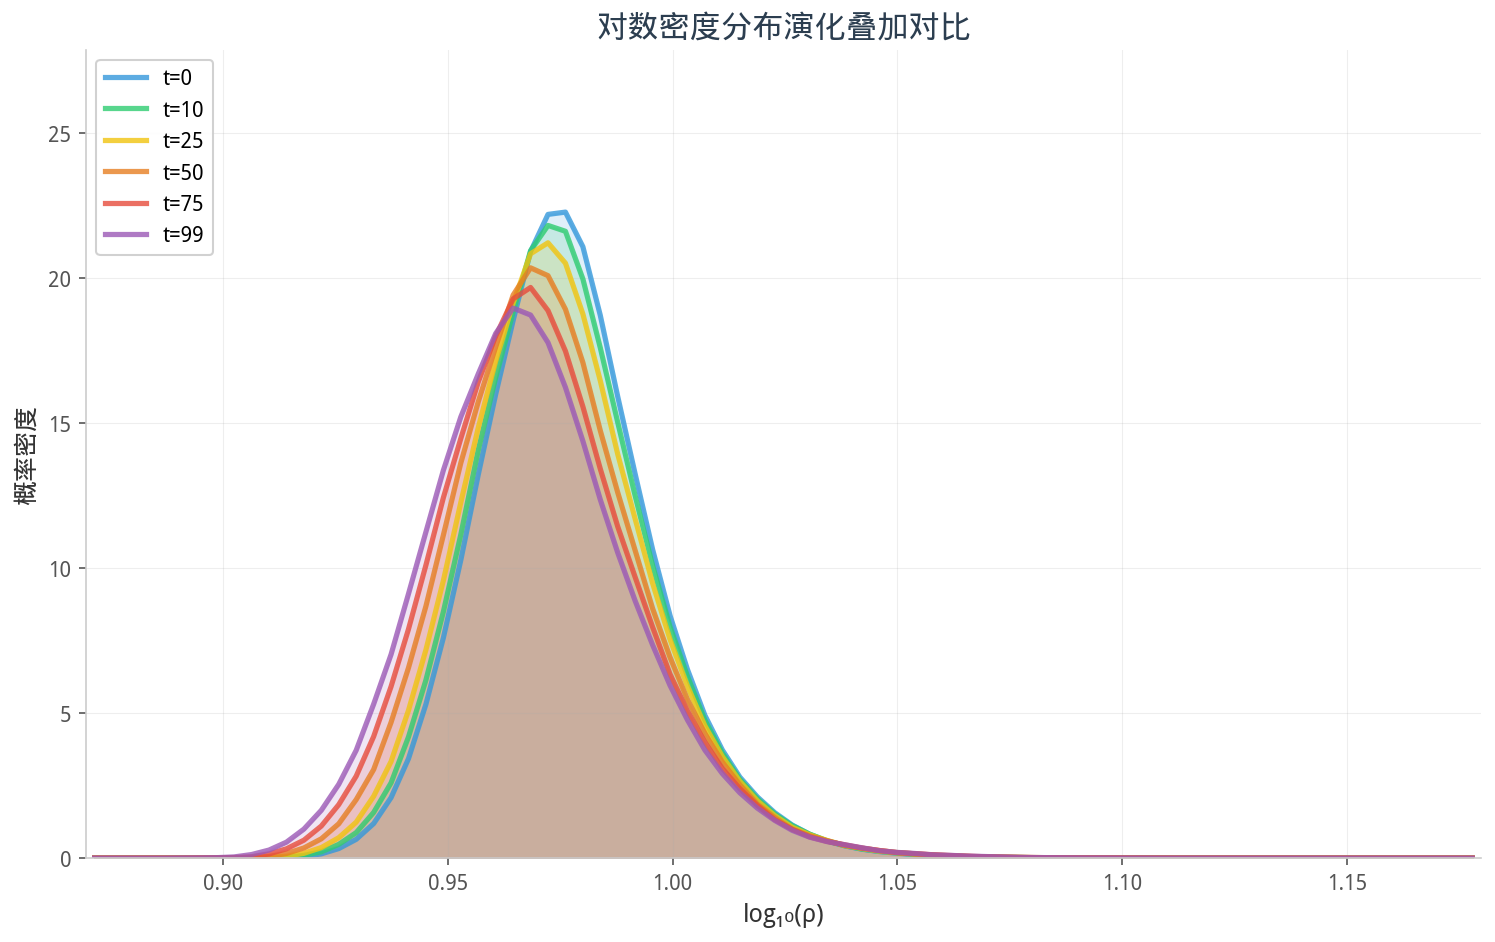
\includegraphics[width=0.90\textwidth]{figures/task3_log_histogram_overlay.png}
    \caption{对数密度分布演化叠加对比：六条曲线展示从窄峰（蓝色,t=0)到宽平台（紫色,t=99)的渐进展宽}
    \label{fig:task3_overlay}
\end{figure}



图 \ref{fig:task3_cdf} 展示了密度累积分布函数(CDF)的时序演化。早期(t=0)曲线陡峭上升，说明大部分体素的密度集中在一个狭窄区间内；晚期(t=99)曲线整体向右上方``拉伸'',中后段变得平缓，意味着更多体素分布在更宽的密度范围内。图中标注的P1、P5、P50、P95、P99分位数以竖线形式呈现:P1与P5(绿色虚线）随时间向左偏移,P95与P99(红色虚线）向右偏移，而P50(黄色虚线）位置相对稳定——这直观地展示了密度分布从中间向两极``撕开''的演化规律。

\begin{figure}[H]
    \centering
    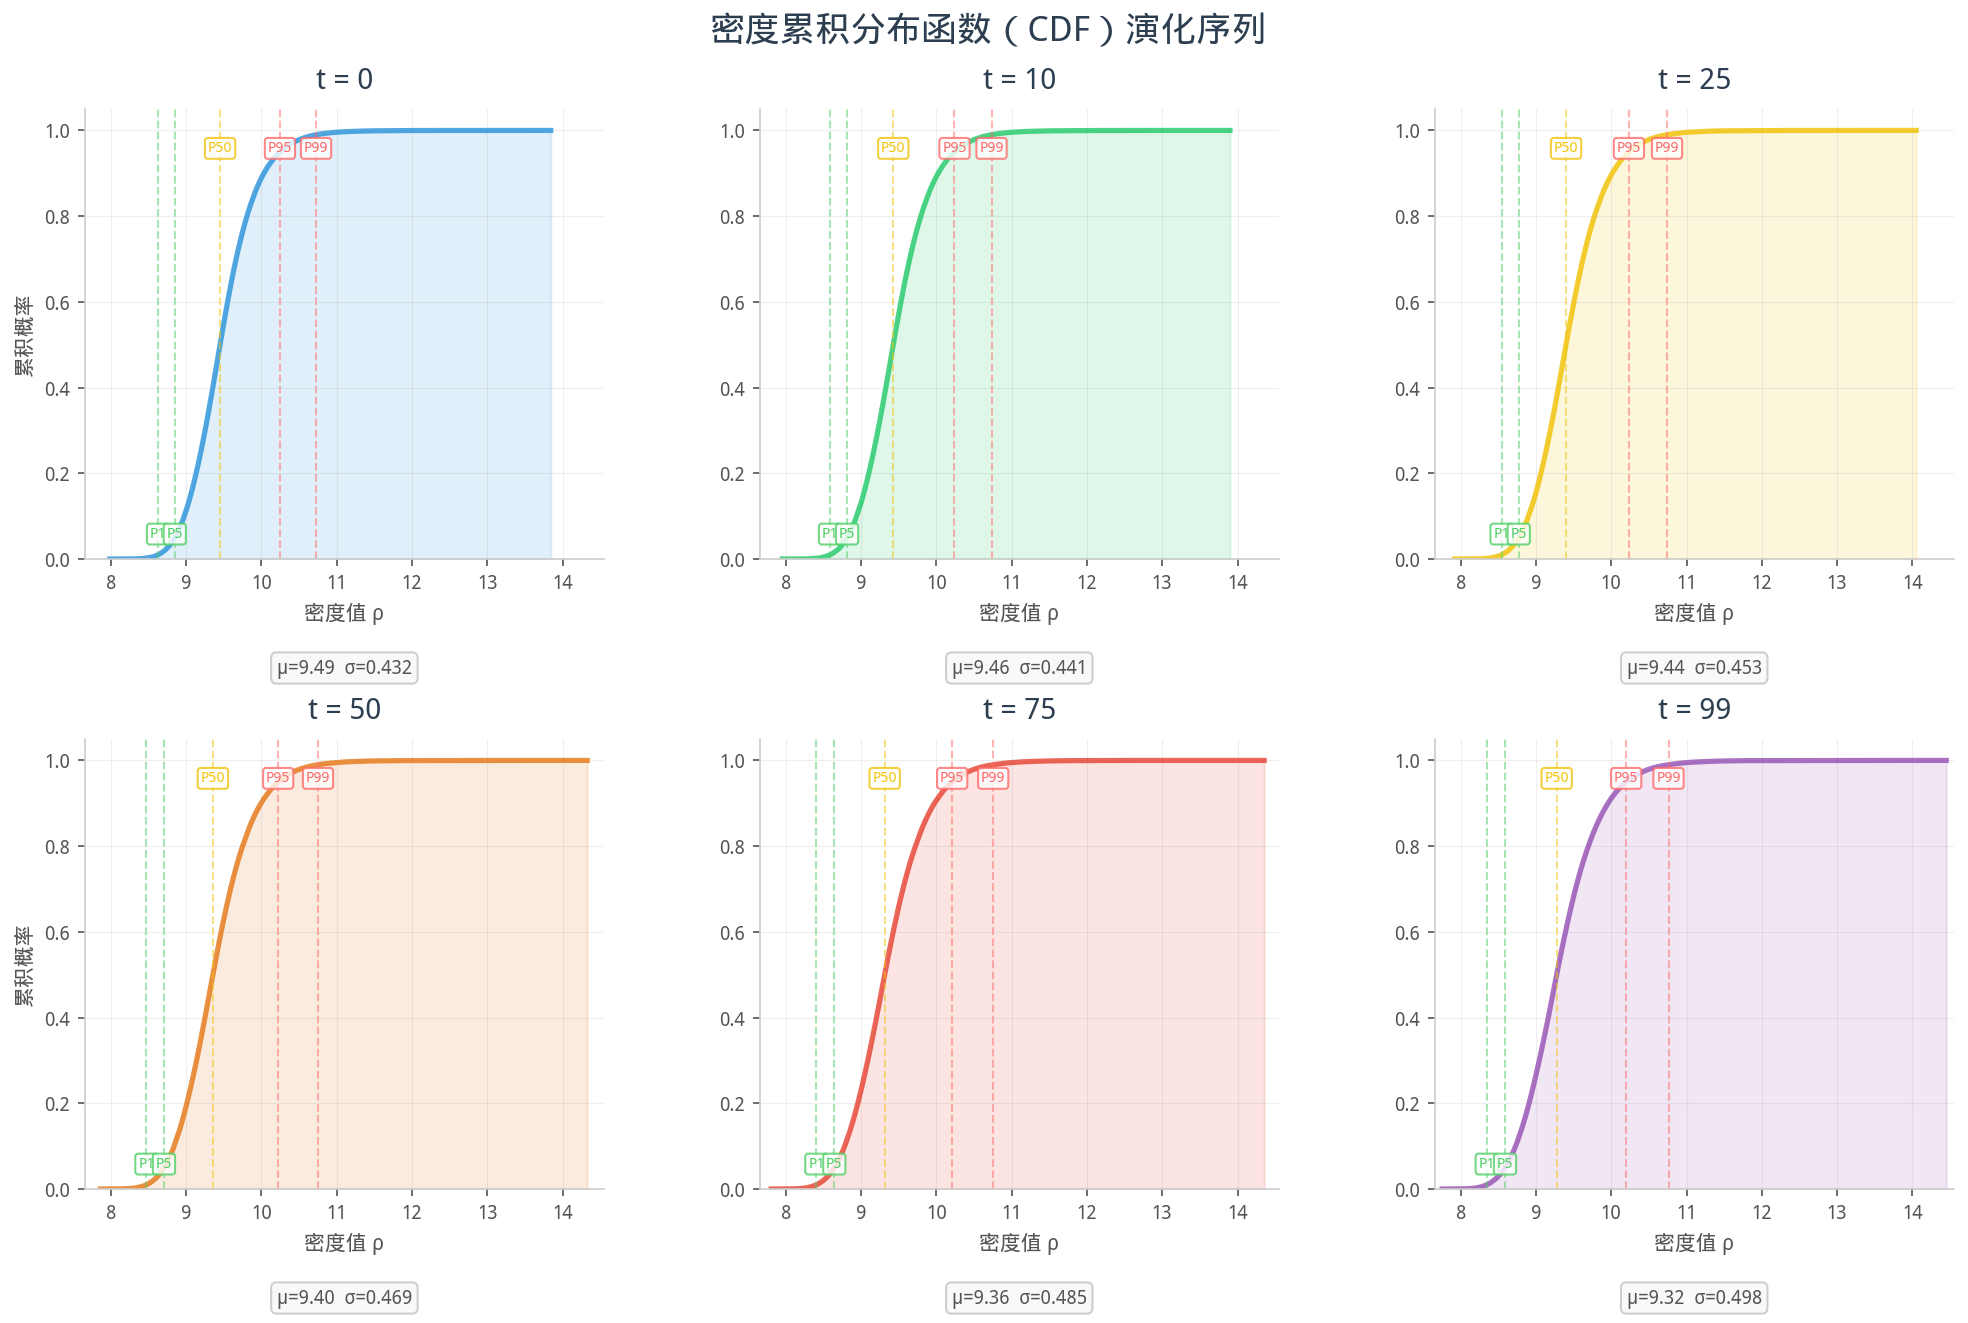
\includegraphics[width=0.95\textwidth]{figures/task3_cdf_sequence.png}
    \caption{密度累积分布函数(CDF)演化序列：标注P1/P5/P50/P95/P99分位数，展示分布随时间的偏移}
    \label{fig:task3_cdf}
\end{figure}

\paragraph{图像生成原理}图 \ref{fig:task3_loghist} 的生成首先选取 t=0、10、25、50、75、99 六个代表性时间步，逐个读取对应的原始 \texttt{.dat} 文件并还原为 $128^3$ 的 NumPy 数组。随后，对每个数组执行 \texttt{flatten()} 展平为一维，再调用 \texttt{np.log10(flat)} 进行常用对数变换，将密度值的指数级动态范围压缩为线性尺度。为了统一对比，先遍历所有六个时间步计算对数密度的全局最小值和最大值，并在此基础上扩展 0.02 的边距作为六张子图共用的横轴范围 \texttt{log\_xlim}。同时，预先计算每个时间步的归一化频数上限，取全局最大值并乘以 1.15 作为统一的纵轴上限，确保六张直方图在相同比例下可直观比较。接着使用 \texttt{plt.subplots(2, 3, figsize=(15, 10))} 创建 2×3 阵列，每个子图以 \texttt{ax.hist} 绘制 60 个分箱的对数密度直方图，启用 \texttt{density=True} 使纵轴表示概率密度而非原始频数。每个子图使用渐变色（蓝、绿、黄、橙、红、紫）区分不同时间步，并通过 \texttt{FormatStrFormatter("\%.4f")} 将横轴刻度精确到四位小数。此外，每个子图底部通过 \texttt{ax.text} 以 \texttt{transAxes} 坐标标注该时刻的均值与标准差，同时在峰值位置用红色圆点标记并标注峰值坐标。

\begin{lstlisting}[language=Python, caption=对数直方图序列图生成关键代码]
steps = [0, 10, 25, 50, 75, 99]
fig, axes = plt.subplots(2, 3, figsize=(15, 10), facecolor='white')
fig.subplots_adjust(left=0.07, right=0.96, top=0.90, bottom=0.10,
                    hspace=0.40, wspace=0.30)
axes_flat = axes.flatten()
all_log_data = []
for ts in steps:
    data = read_raw_dat(DATA_DIR / f"{ts:04d}.dat")
    flat = data.flatten()
    log_flat = np.log10(flat)
    all_log_data.append(log_flat)
log_min = min(np.min(d) for d in all_log_data)
log_max = max(np.max(d) for d in all_log_data)
log_xlim = (log_min - 0.02, log_max + 0.02)
global_ymax = 0
for log_flat in all_log_data:
    n, _ = np.histogram(log_flat, bins=60, range=log_xlim, density=True)
    global_ymax = max(global_ymax, max(n))
colors = ['#3498DB', '#2ECC71', '#F1C40F', '#E67E22', '#E74C3C', '#9B59B6']
for i, (ts, log_flat) in enumerate(zip(steps, all_log_data)):
    ax = axes_flat[i]
    ax.set_facecolor('white')
    n, bins, patches = ax.hist(log_flat, bins=60, range=log_xlim,
                                 color=colors[i], edgecolor='white',
                                 alpha=0.85, density=True, linewidth=0.3)
    ax.set_xlim(log_xlim)
    ax.set_ylim(0, global_ymax * 1.15)
    ax.set_title(f't = {ts}', fontsize=14, fontweight='bold',
                 color='#2C3E50', pad=10)
    ax.set_xlabel('log₁₀(ρ)', fontsize=11, color='#555555')
    if i % 3 == 0:
        ax.set_ylabel('概率密度', fontsize=11, color='#555555')
    ax.xaxis.set_major_formatter(FormatStrFormatter(r"%.4f"))
    ax.tick_params(axis='both', labelsize=9, colors='#555555')
    ax.spines['bottom'].set_color('#CCCCCC')
    ax.spines['left'].set_color('#CCCCCC')
    ax.spines['top'].set_visible(False)
    ax.spines['right'].set_visible(False)
    ax.grid(True, alpha=0.2, color='#AAAAAA', linestyle='-', linewidth=0.5)
    flat = np.power(10, log_flat)
    mean_val = np.mean(flat)
    std_val = np.std(flat)
    ax.text(0.5, -0.22, f'μ={mean_val:.2f}  σ={std_val:.3f}',
            transform=ax.transAxes, fontsize=9, ha='center', va='top',
            color='#555555',
            bbox=dict(boxstyle='round,pad=0.3', facecolor='#F8F9FA',
                      edgecolor='#CCCCCC', alpha=0.95))
    peak_idx = np.argmax(n)
    peak_x = (bins[peak_idx] + bins[peak_idx + 1]) / 2
    peak_y = n[peak_idx]
    ax.plot(peak_x, peak_y, 'o', color='#E74C3C', markersize=6,
            markeredgecolor='white', markeredgewidth=1, zorder=5)
    ax.text(peak_x, peak_y + global_ymax * 0.08, f'峰:{peak_x:.3f}',
            ha='center', fontsize=8, color='#E74C3C', fontweight='bold',
            bbox=dict(boxstyle='round,pad=0.2', facecolor='white',
                      edgecolor='#E74C3C', alpha=0.9))
fig.suptitle('密度对数直方图演化序列', fontsize=17, fontweight='bold',
             color='#2C3E50', y=0.97)
plt.savefig(OUT_DIR / 'task3_log_histogram_sequence.png', dpi=150,
            bbox_inches='tight', facecolor='white', edgecolor='none')
plt.close()
\end{lstlisting}



图 \ref{fig:task3_overlay} 的生成基于同一批对数密度数据。对每个时间步，先调用 \texttt{np.histogram(log\_flat, bins=80, range=log\_xlim, density=True)} 计算归一化频数，再取相邻分箱边界的平均值作为曲线中心点。随后，使用 \texttt{ax.plot} 在同一坐标系上绘制六条概率密度曲线，每条曲线使用与图 \ref{fig:task3_loghist} 对应的渐变色，线宽设为 2.5 像素，并通过 \texttt{fill\_between} 在曲线下方填充同色半透明区域（透明度 0.15）。纵轴上限设为全局最大概率密度的 1.25 倍，确保曲线之间不重叠遮挡。图例置于左上角，背景透明度设为 0.9，最后以 150 DPI 输出 PNG 文件。

\begin{lstlisting}[language=Python, caption=对数密度叠加对比图生成关键代码]
fig2, ax2 = plt.subplots(figsize=(12, 7), facecolor='white')
ax2.set_facecolor('white')
for i, (ts, log_flat) in enumerate(zip(steps, all_log_data)):
    n, bins = np.histogram(log_flat, bins=80, range=log_xlim, density=True)
    centers = (bins[:-1] + bins[1:]) / 2
    ax2.plot(centers, n, color=colors[i], lw=2.5, label=f't={ts}', alpha=0.8)
    ax2.fill_between(centers, n, alpha=0.15, color=colors[i])
ax2.set_xlim(log_xlim)
ax2.set_ylim(0, global_ymax * 1.25)
ax2.set_xlabel('log₁₀(ρ)', fontsize=12, color='#333333')
ax2.set_ylabel('概率密度', fontsize=12, color='#333333')
ax2.set_title('对数密度分布演化叠加对比', fontsize=15, fontweight='bold',
               color='#2C3E50')
ax2.legend(loc='upper left', fontsize=10, framealpha=0.9)
ax2.tick_params(axis='both', labelsize=10, colors='#555555')
ax2.spines['bottom'].set_color('#CCCCCC')
ax2.spines['left'].set_color('#CCCCCC')
ax2.spines['top'].set_visible(False)
ax2.spines['right'].set_visible(False)
ax2.grid(True, alpha=0.2, color='#AAAAAA', linestyle='-', linewidth=0.5)
plt.savefig(OUT_DIR / 'task3_log_histogram_overlay.png', dpi=150,
            bbox_inches='tight', facecolor='white', edgecolor='none')
plt.close()
\end{lstlisting}



图 \ref{fig:task3_cdf} 的生成同样基于六个时间步的原始密度数据。对每个时间步，先将密度值展平为一维数组，再调用 \texttt{np.sort(flat)} 进行升序排序，随后计算累积概率序列 \texttt{np.arange(1, len(sorted\_data)+1) / len(sorted\_data)}，即每个排序位置对应的比例累积值。使用 \texttt{ax.plot(sorted\_data, cdf)} 绘制 CDF 曲线，并在曲线下方填充同色半透明区域。关键分位数通过 \texttt{np.percentile(flat, p)} 计算，其中 P1 和 P5 以绿色虚线标注、P50 以黄色虚线标注、P95 和 P99 以红色虚线标注；每条虚线旁通过 \texttt{ax.text} 添加带圆角边框的文本标签 \texttt{P1}、\texttt{P5} 等。六张 CDF 子图同样采用 2×3 阵列布局，统一横轴范围由全局最小和最大密度值确定，纵轴固定为 0--1.05，底部标注均值与标准差。整体以 150 DPI 保存为 PNG 文件。


\begin{lstlisting}[language=Python, caption=CDF演化序列图生成关键代码]
steps = [0, 10, 25, 50, 75, 99]
fig, axes = plt.subplots(2, 3, figsize=(14, 9), facecolor='white')
fig.subplots_adjust(left=0.07, right=0.96, top=0.90, bottom=0.10,
                    hspace=0.40, wspace=0.30)
axes_flat = axes.flatten()
colors = ['#3498DB', '#2ECC71', '#F1C40F', '#E67E22', '#E74C3C', '#9B59B6']
all_data = []
for ts in steps:
    data = read_raw_dat(DATA_DIR / f"{ts:04d}.dat")
    all_data.append(data.flatten())
global_xlim = (min(d.min() for d in all_data) - 0.1,
               max(d.max() for d in all_data) + 0.1)
for i, (ts, flat) in enumerate(zip(steps, all_data)):
    ax = axes_flat[i]
    ax.set_facecolor('white')
    sorted_data = np.sort(flat)
    cdf = np.arange(1, len(sorted_data) + 1) / len(sorted_data)
    ax.plot(sorted_data, cdf, color=colors[i], lw=2.5, alpha=0.85)
    ax.fill_between(sorted_data, cdf, alpha=0.15, color=colors[i])
    for p, color_p in [(1, '#51cf66'), (5, '#51cf66'), (50, '#f1c40f'),
                       (95, '#ff6b6b'), (99, '#ff6b6b')]:
        val = np.percentile(flat, p)
        ax.axvline(val, color=color_p, linestyle='--', alpha=0.5, lw=1)
        ax.text(val, 0.05 if p < 50 else 0.95, f'P{p}',
                ha='center', fontsize=7, color=color_p, fontweight='bold',
                bbox=dict(boxstyle='round,pad=0.2', facecolor='white',
                          edgecolor=color_p, alpha=0.8))
    ax.set_xlim(global_xlim)
    ax.set_ylim(0, 1.05)
    ax.set_title(f't = {ts}', fontsize=14, fontweight='bold',
                 color='#2C3E50', pad=10)
    ax.set_xlabel('密度值 ρ', fontsize=10, color='#555555')
    if i % 3 == 0:
        ax.set_ylabel('累积概率', fontsize=10, color='#555555')
    ax.tick_params(axis='both', labelsize=9, colors='#555555')
    ax.spines['bottom'].set_color('#CCCCCC')
    ax.spines['left'].set_color('#CCCCCC')
    ax.spines['top'].set_visible(False)
    ax.spines['right'].set_visible(False)
    ax.grid(True, alpha=0.2, color='#AAAAAA', linestyle='-', linewidth=0.5)
    mean_val = np.mean(flat)
    std_val = np.std(flat)
    ax.text(0.5, -0.22, f'μ={mean_val:.2f}  σ={std_val:.3f}',
            transform=ax.transAxes, fontsize=9, ha='center', va='top',
            color='#555555',
            bbox=dict(boxstyle='round,pad=0.3', facecolor='#F8F9FA',
                      edgecolor='#CCCCCC', alpha=0.95))
fig.suptitle('密度累积分布函数（CDF）演化序列', fontsize=17, fontweight='bold',
             color='#2C3E50', y=0.97)
plt.savefig(OUT_DIR / 'task3_cdf_sequence.png', dpi=150,
            bbox_inches='tight', facecolor='white', edgecolor='none')
plt.close()
\end{lstlisting}




%========================================
\section{任务四}
%========================================

\paragraph{问题}
相空间交互式刷选可视分析：搭建联动式交互可视分析仪表盘，实现基于相空间的筛选分析功能。支持用户在统计直方图中自定义框选特定密度区间，例如筛选占比1\%的极高密度区间。系统可实时联动三维空间视图，快速渲染匹配该密度阈值的物理单元格数据，直观验证直方图高密度尾部数据与宇宙网节点致密结构的对应关系，实现统计特征与空间物理结构的双向关联分析。

\paragraph{回答}

图 \ref{fig:task4_brush} 展示了在密度分布直方图中框选 Top 1\% 高密度区间的操作结果。图中直方图右尾有一块明显的蓝色虚线框选区域，对应筛选区间 [10.73, 13.84],体素占比 1.08\%。从统计角度看，这些体素位于整个密度分布的最右端尾部，密度值远高于均值(9.395),属于极端高密度样本。

\begin{figure}[htbp]
    \centering
    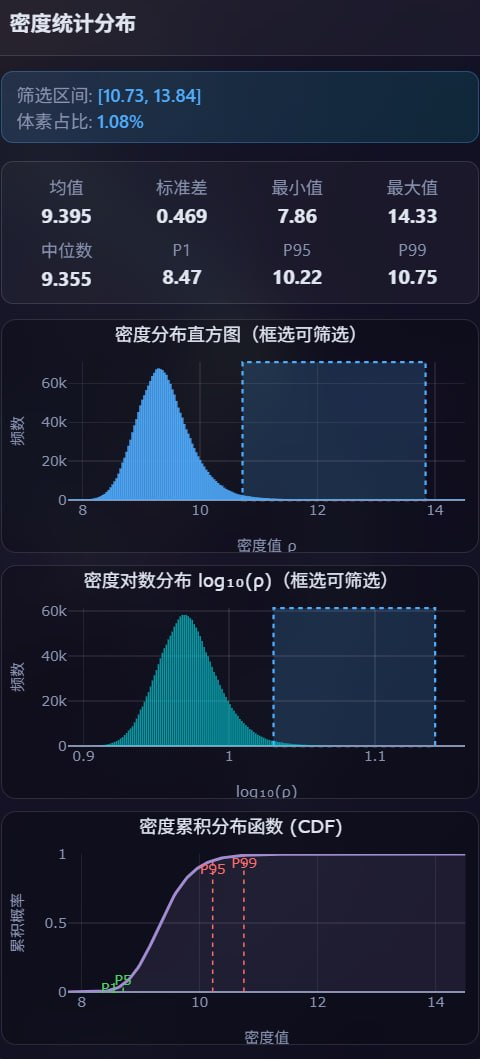
\includegraphics[width=0.85\textwidth,height=0.9\textheight,keepaspectratio]{figures/task4_histogram_brush.jpg}
    \caption{直方图框选操作：蓝色虚线框标注 Top 1\% 高密度区间，筛选区间 [10.73, 13.84],体素占比 1.08\%}
    \label{fig:task4_brush}
\end{figure}

当系统将低于阈值的体素全部透明化后，图 \ref{fig:task4_top1} 展示了仅保留 Top 1\% 高密度体素的三维渲染结果。原本连续弥漫的密度场被``剥离''后，空间中只剩下若干离散的亮白色团块，这些团块在黑色背景中呈节点状散布，彼此之间隐约可见暗弱的丝状连接。这种空间分布形态与宇宙网理论中的``节点——纤维''拓扑高度吻合，初步验证了：直方图右尾的高密度尾部在三维空间中确实对应着致密的节点结构。

\begin{figure}[htbp]
    \centering
    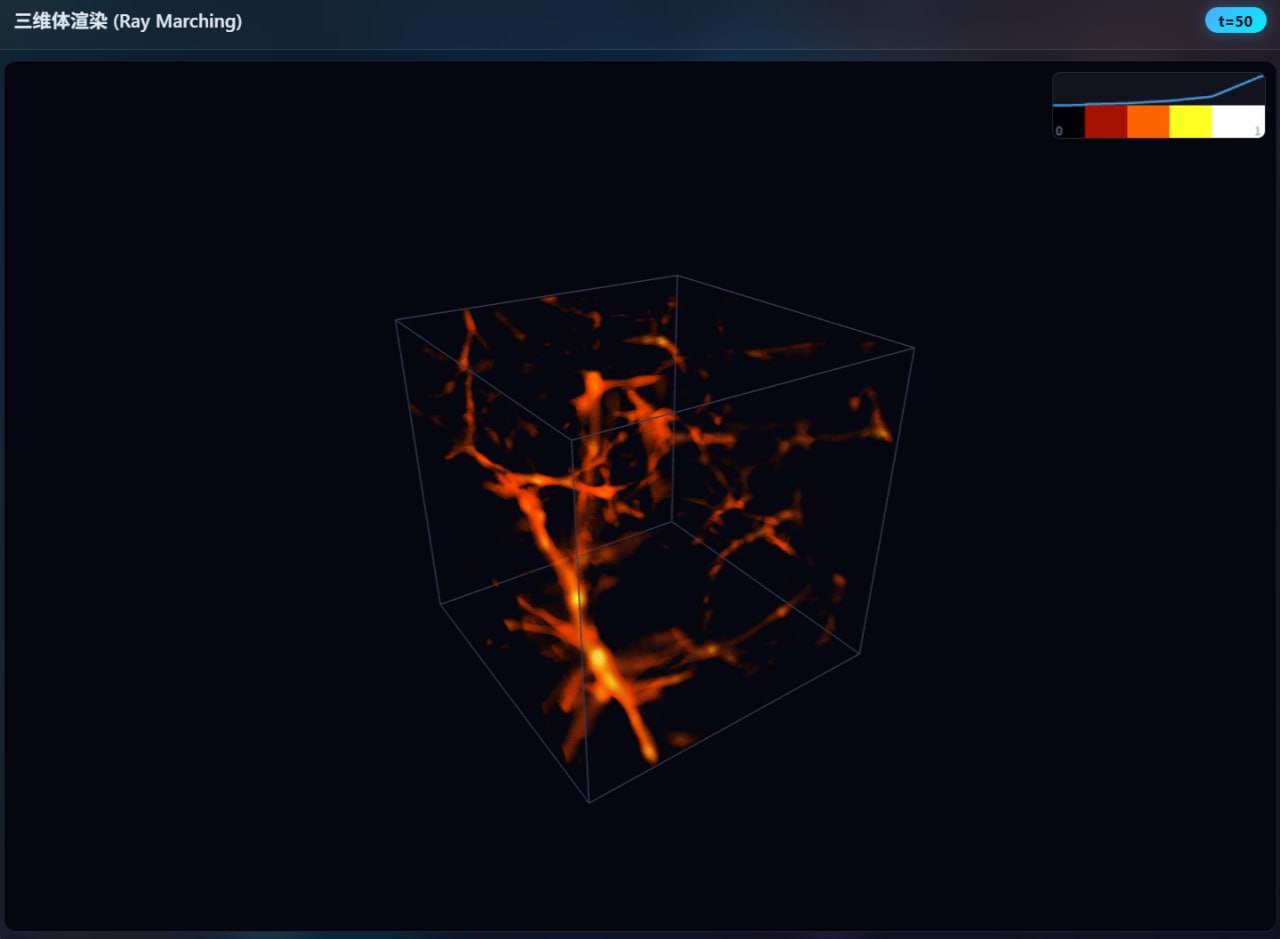
\includegraphics[width=0.80\textwidth]{figures/task4_top1_3d.jpg}
    \caption{Top 1\% 高密度体素三维渲染(t=50):仅显示密度 $\ge$ P99 的体素，亮白色团块对应宇宙网致密节点}
    \label{fig:task4_top1}
\end{figure}

图 \ref{fig:task4_p95} 将筛选阈值从 P99 放宽至 P95(Top 5\%),展示了同一时刻的三维渲染结果。与图 \ref{fig:task4_top1} 相比，三维视图中除保留原有的亮斑节点外，还显现出大量连接节点的丝状结构——这些中等密度的体素在 P99 筛选下被透明化，但在 P95 筛选下得以保留，恰好对应宇宙网理论中连接节点的纤维(filaments)。这说明直方图右尾不同区段对应着不同的空间拓扑层次:P99 以上对应致密节点,P95--P99 区间对应连接丝，而密度更低的区域则对应片状结构与广阔空洞。通过调整筛选阈值，研究者可以像``剥洋葱''一样逐层揭示宇宙网的四级拓扑结构。

\begin{figure}[htbp]
    \centering
    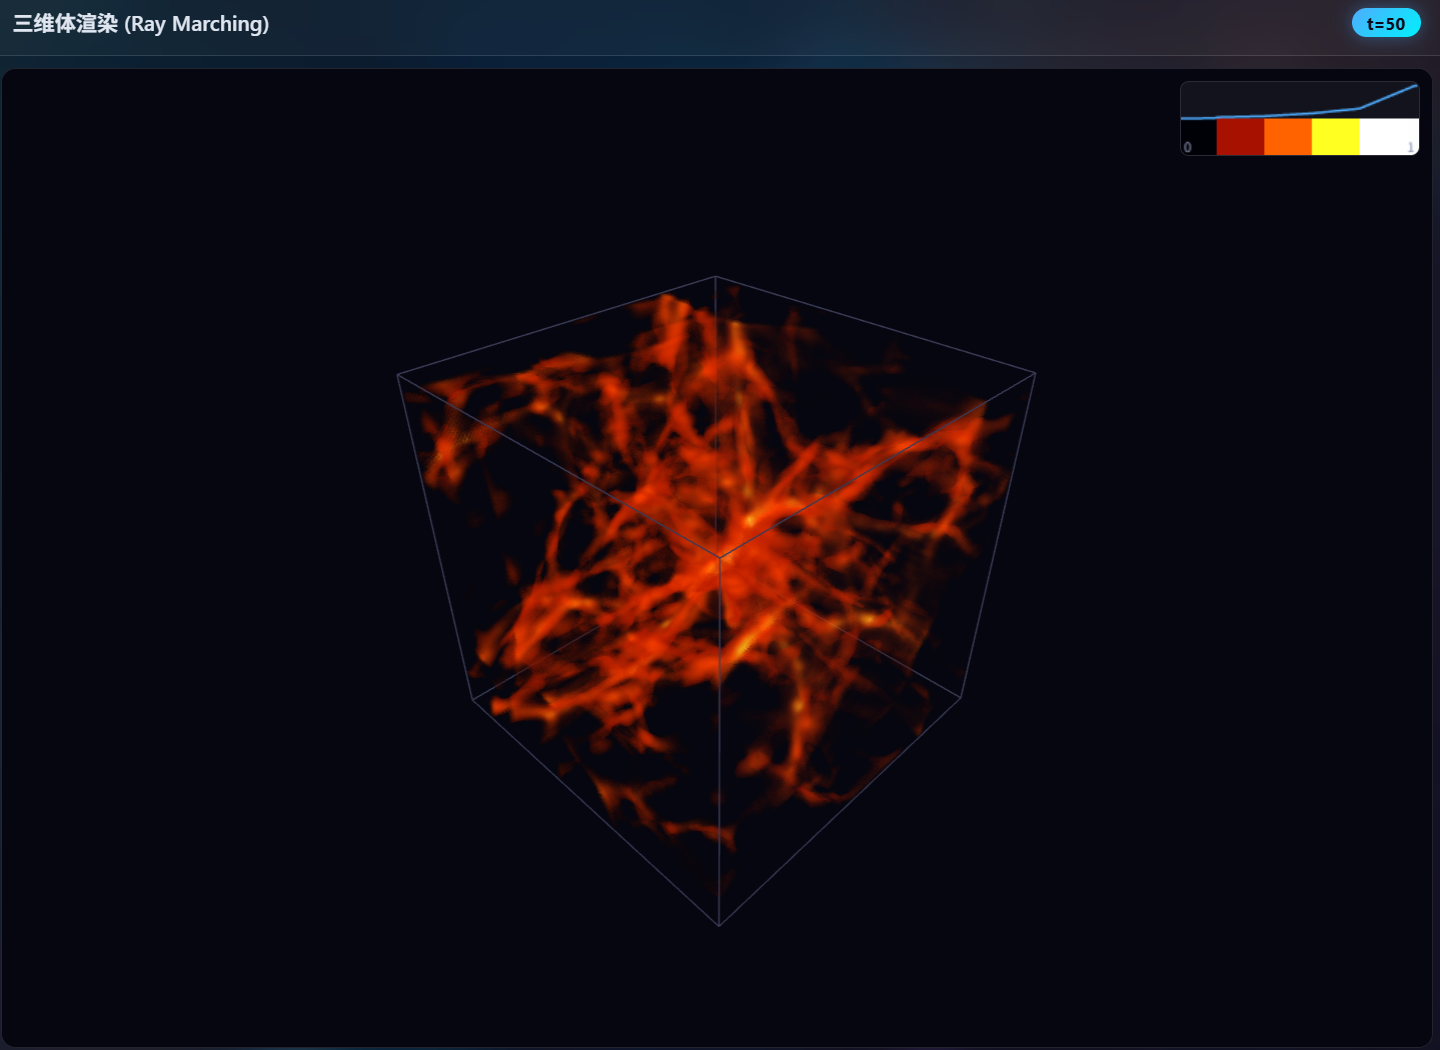
\includegraphics[width=0.75\textwidth]{figures/task4_t50_p95.png}
    \caption{Top 5\% 高密度体素三维渲染(t=50,P95 阈值):亮斑节点外显现连接丝状结构}
    \label{fig:task4_p95}
\end{figure}

图 \ref{fig:task4_t99} 展示了晚期(t=99)Top 1\% 筛选的三维渲染结果。与 t=50 相比,t=99 的亮斑团块数量更多、分布更密集，丝状连接更清晰，整体网络结构更加成熟——这反映了晚期宇宙网中晕的并合与纤维的持续吸积。晚期节点亮度更高，说明经过额外 49 个时间步的引力坍缩，晕核密度进一步增大，对应直方图尾端向更高密度值延伸。这种时序对比表明，统计尾部的位置随时间向高密度方向漂移，与三维空间中节点结构的持续致密化完全同步。

\begin{figure}[htbp]
    \centering
    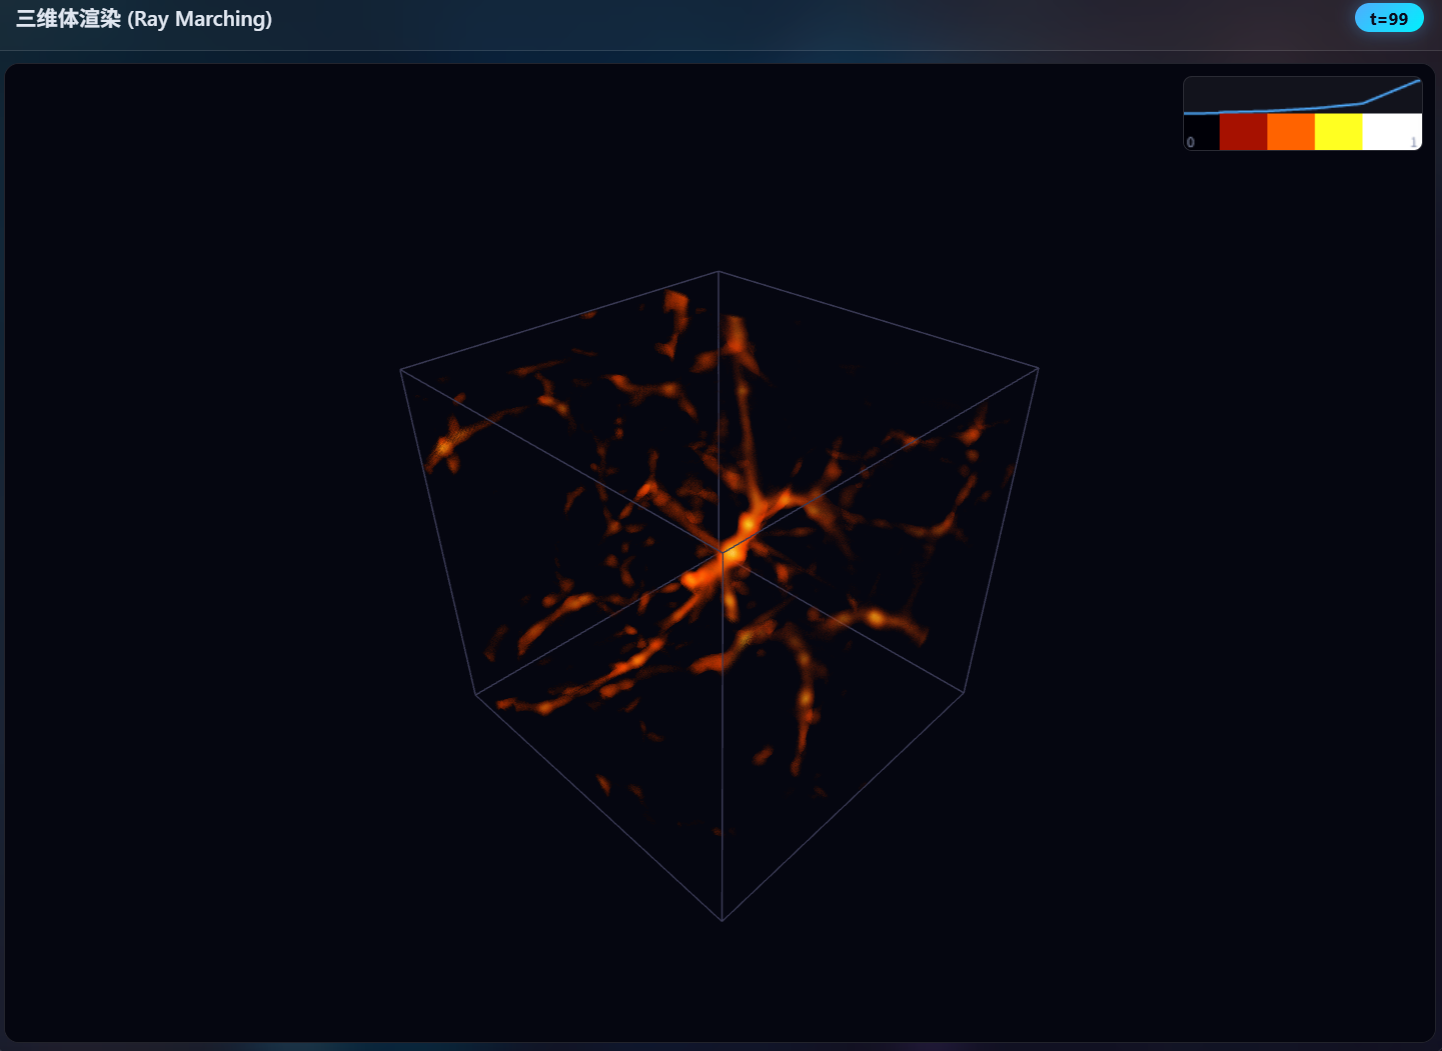
\includegraphics[width=0.75\textwidth]{figures/task4_t99_p99.png}
    \caption{Top 1\% 高密度体素三维渲染(t=99,P99 阈值):晚期宇宙网节点更密集、网络更成熟}
    \label{fig:task4_t99}
\end{figure}

图 \ref{fig:task4_aip} 展示了同一时刻(t=50)采用平均强度投影(AIP)而非最大强度投影(MIP)的三维渲染结果。AIP 保留视线方向上的整体密度加权平均，而非仅取最大值，因此渲染结果呈弥漫性的云雾状填充，丝状结构边界模糊但连续性更强，更适合观察大尺度气体的整体分布特征。与图 \ref{fig:task4_p95} 的 MIP 骨架视图形成功能互补:MIP 突出拓扑骨架节点,AIP 展示气体填充全貌。两种投影方法的联合使用，使研究者既能定位高密度节点，又能理解周围气体的分布环境。

\begin{figure}[htbp]
    \centering
    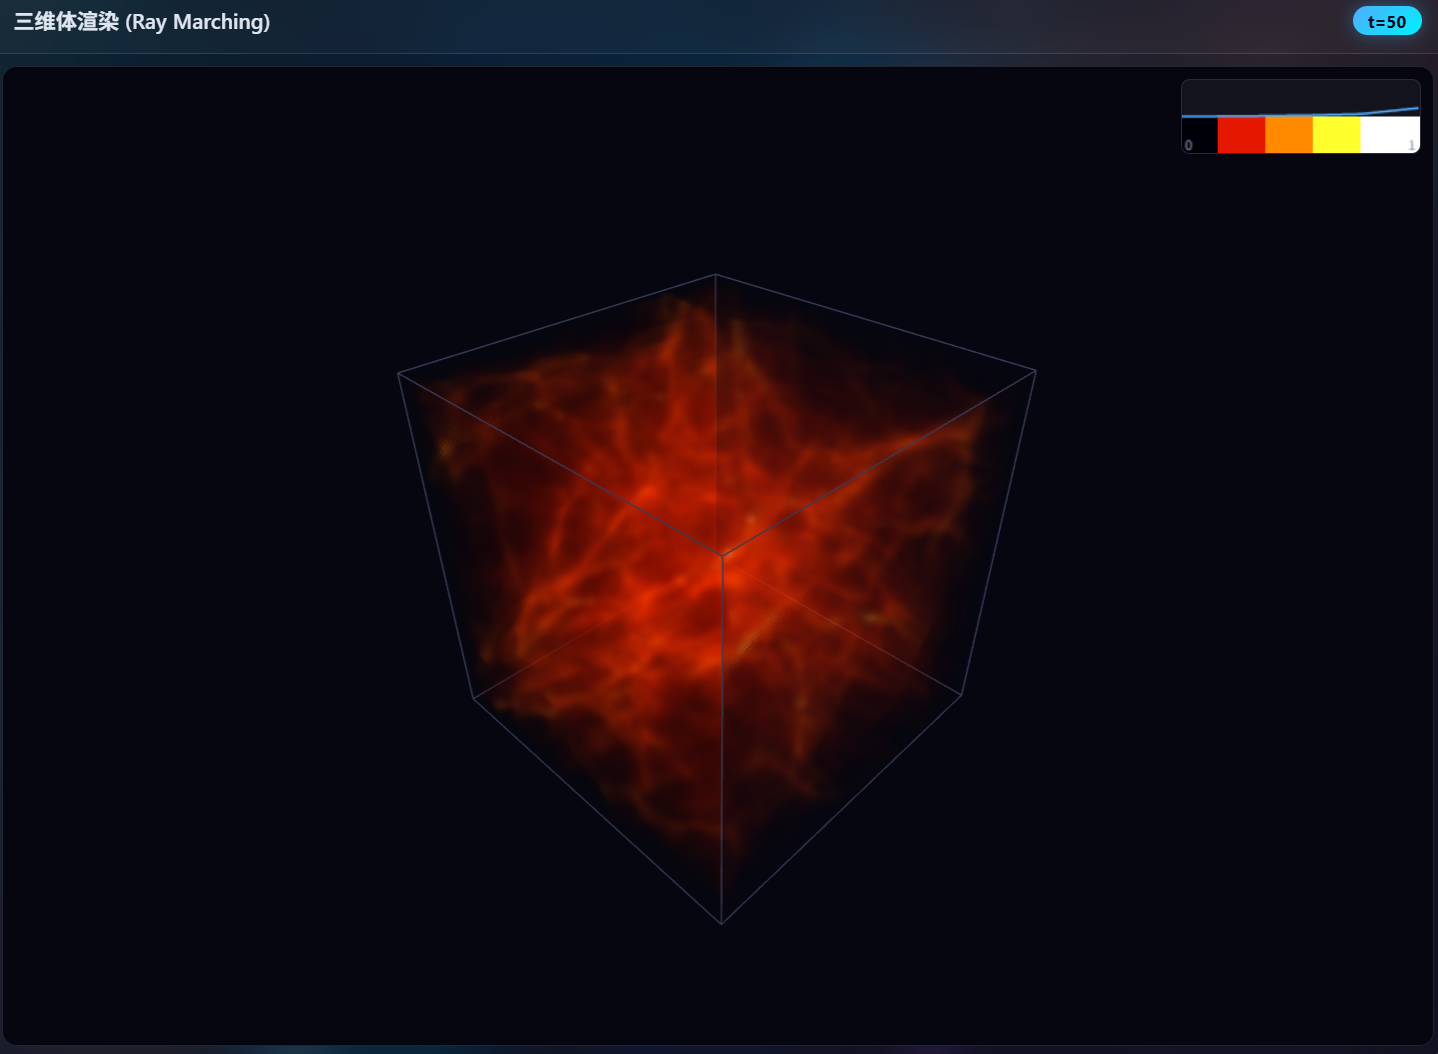
\includegraphics[width=0.75\textwidth]{figures/task4_t50_aip.png}
    \caption{平均强度投影(AIP)三维渲染(t=50,无筛选):弥漫性云雾状气体填充，展示大尺度密度场全貌}
    \label{fig:task4_aip}
\end{figure}

综上所述，通过直方图框选与三维体渲染的联动分析，可以得出以下结论。第一，直方图高密度尾部数据与宇宙网节点致密结构之间存在精确的定量对应关系：密度分布最右端约 1\% 的体素（密度 $\ge$ P99)在三维空间中聚集成离散的亮斑团块，这些团块正是引力坍缩形成的暗物质晕核心。第二，不同筛选阈值对应不同的空间拓扑层次--P99 见节点,P95 见纤维丝，更宽的区间则见片状结构与空洞，实现了从统计数值到空间结构的逐层解码。第三，时序对比验证了这种对应关系的动态演化：晚期节点更密集、更明亮，与统计尾部向高密度漂移同步。第四,MIP 与 AIP 两种投影方法形成功能互补，前者突出拓扑骨架，后者展示气体填充全貌。通过联动式刷选技术，用户在直方图中框选任意密度区间即可实时在三维空间中定位对应的物理结构，反之亦可通过空间结构的密度值反推其在统计分布中的位置，从而完整实现了统计特征与空间物理结构的双向关联分析。

\paragraph{制作原理}任务四交互式仪表盘采用 Flask 后端架构（前后端不分离），通过 Python 模板渲染直接生成单页面 HTML。前端核心渲染层基于 Three.js 和 WebGL 2.0 实现自定义 Ray Marching 实时光线投射体渲染。具体而言，预降采样至 $64^3$ 的 \texttt{uint8} 体数据由后端以二进制流形式传输，前端通过 \texttt{THREE.DataTexture3D} 将其上传为 GPU 3D 纹理，随后在片元着色器中执行完整的射线-包围盒求交与发射-吸收光学积分。着色器内部支持 MIP（最大强度投影）与 AIP（平均强度投影）两种积分模式的动态切换：MIP 模式下沿视线方向取体素最大值，突出高密度骨架结构；AIP 模式下沿视线方向累加密度值并除以采样步数，保留整体密度加权平均。此外，着色器内置五种传递函数预设（Hot / Cool / Fire / Rainbow / yt Log-Layers），通过 1D 纹理查找表将原始密度值映射为 RGBA 颜色；对数映射模式则通过在着色器内执行 \texttt{log} 变换拉开低密度区域动态范围，增强宇宙空洞结构的可分辨性。不透明度（默认 1.2）与亮度（默认 1.8）通过 Uniform 变量实时传入，采样步数（低/中/高三档）控制光线投射的密度与渲染质量。

右侧统计面板基于 Plotly.js 绘制交互式直方图、对数直方图与累积分布函数（CDF）。当用户在直方图中执行鼠标框选（Brush）时，Plotly 触发 \texttt{plotly\_selected} 事件，前端 JavaScript 通过事件回调捕获所选密度区间的 \texttt{xRange} 上下界。该区间值被写入全局 Vue 状态对象，并同步触发 Three.js 体渲染材质的 Uniform 更新：\texttt{thresholdMin} 和 \texttt{thresholdMax} 分别设为所选区间的下界和上界，片元着色器在采样时通过条件判断将区间外体素的 Alpha 值置零，从而实现仅高亮显示选中密度区间的物理单元格。反之，当用户通过底部密度滑块或预设按钮（Top 1\% / 5\% / 10\%）调整阈值时，JavaScript 同步更新 Plotly 图表的框选范围，完成统计直方图与三维空间视图的双向联动。密度筛选预设的计算逻辑基于预计算的 \texttt{stats.json} 分位数数据，Top 1\% 对应 P99 阈值，Top 5\% 对应 P95 阈值，Top 10\% 对应 P90 阈值。

数据层的构建由后端 Python 脚本 \texttt{preprocess\_web\_data.py} 完成。该脚本遍历 100 个时间步，逐个读取原始 $128^3$ 密度场，沿 X、Y、Z 三个轴分别计算 MIP 和 AIP 投影，并通过 Matplotlib 以 64 DPI 输出为小型 PNG 文件（共 600 张），供前端在二维切面面板中即时加载。同时，脚本将原始数据降采样至 $64^3$ 的 \texttt{uint8} 体数据并保存为二进制文件，供 WebGL 3D 纹理直接使用。\texttt{stats.json} 和 \texttt{histograms.json} 则从预处理目录复制至 Web 静态资源目录，作为前端 Plotly 图表的数据源。这种预计算策略确保前端仪表盘在切换时间步或调整视角时无需重复计算，从而实现流畅的实时交互体验。

\begin{lstlisting}[language=Python, caption=Web 预渲染数据生成脚本]
import numpy as np, json, shutil, struct
from pathlib import Path
import matplotlib
matplotlib.use('Agg')
import matplotlib.pyplot as plt

DATA_DIR = Path("./data/Nyx")
PROCESSED_DIR = Path("./data/processed")
WEB_DATA_DIR = Path("./web/static/data")
PROJECTIONS_DIR = WEB_DATA_DIR / "projections"
PROJECTIONS_DIR.mkdir(parents=True, exist_ok=True)
WEB_DATA_DIR.mkdir(parents=True, exist_ok=True)

NX, NY, NZ = 128, 128, 128
NTOTAL = 100

def read_raw_dat(filepath):
    with open(filepath, 'rb') as f:
        raw = f.read()
    n_floats = len(raw) // 4
    data = struct.unpack('<' + 'f' * n_floats, raw)
    return np.array(data, dtype=np.float32).reshape((NX, NY, NZ))

def compute_projection(field, axis, proj_type='mip'):
    if proj_type == 'mip':
        return np.max(field, axis=axis)
    elif proj_type == 'aip':
        return np.mean(field, axis=axis)
    else:
        raise ValueError(f"Unknown projection type: {proj_type}")

def save_projection_png(data, filepath):
    fig, ax = plt.subplots(figsize=(2.5, 2.5), dpi=64)
    im = ax.imshow(data, cmap='hot', origin='lower', aspect='auto')
    ax.axis('off')
    plt.subplots_adjust(left=0, right=1, bottom=0, top=1)
    fig.savefig(filepath, dpi=64, bbox_inches='tight', pad_inches=0,
                facecolor='black', edgecolor='none')
    plt.close(fig)

def main():
    print(f"开始预处理 {NTOTAL} 个时间步的投影图...")
    for ts in range(NTOTAL):
        dat_path = DATA_DIR / f"{ts:04d}.dat"
        if not dat_path.exists():
            print(f"  跳过 t={ts} (文件不存在)")
            continue
        field = read_raw_dat(dat_path)
        for axis in range(3):
            axis_name = ['x', 'y', 'z'][axis]
            mip = compute_projection(field, axis, 'mip')
            mip_path = PROJECTIONS_DIR / f"mip_{axis_name}_{ts:04d}.png"
            save_projection_png(mip, mip_path)
            aip = compute_projection(field, axis, 'aip')
            aip_path = PROJECTIONS_DIR / f"aip_{axis_name}_{ts:04d}.png"
            save_projection_png(aip, aip_path)
        if ts % 10 == 0:
            print(f"  已处理 t={ts}")
    # 复制统计数据到 web 目录
    for fname in ['stats.json', 'histograms.json']:
        src = PROCESSED_DIR / fname
        dst = WEB_DATA_DIR / fname
        if src.exists():
            shutil.copy2(src, dst)
            print(f"已复制 {fname} -> {dst}")
    print(f"\n完成！共生成 {NTOTAL * 6} 个 PNG 文件")

if __name__ == '__main__':
    main()
\end{lstlisting}

\section{实验总结}

在本次基于 Nyx 宇宙学模拟数据的交互式可视化分析实验中，整个研究链条从原始二进制数据的解析到最终的 Web 联动仪表盘部署，经历了多个关键阶段，也遇到了若干技术难题，以下从问题、解决方案与收获三个维度进行总结。

\paragraph{遇到的问题与解决方案}

第一，原始数据格式解析困难。Nyx 模拟输出的 \texttt{.dat} 文件为纯二进制 \texttt{float32} 小端序格式，没有头部元信息（如维度、字节序、数据类型标签），直接使用 \texttt{np.fromfile} 默认参数读取会导致数值严重失真。解决方案是先用 Python 的 \texttt{struct} 模块以 \texttt{'<f'} 格式显式解析小端序浮点，确认数据长度为 $128^3$ 后再 \texttt{reshape} 为三维张量，并封装为 \texttt{read\_raw\_dat} 复用函数，确保后续所有脚本使用同一解析标准。

第二，密度动态范围过大导致可视化细节丢失。原始密度值跨越多个数量级，早期与晚期时间步的直方图在原始尺度下几乎无法对比，低密度区域的空洞结构被压缩到不可分辨。解决方案是引入对数变换（\texttt{np.log10}）压缩指数级差异，将动态范围映射到线性尺度；同时在前端 WebGL 着色器中增加对数映射开关，通过着色器内 \texttt{log} 运算实时拉开低密度区域对比度，使宇宙空洞结构在体渲染中清晰可见。

第三，Web 前端实时体渲染性能瓶颈。$128^3$ 体数据直接上传 GPU 进行光线投射，在普通笔记本上帧率极低，且每次切换时间步或调整视角都需要重新计算投影。解决方案是预计算降采样：后端脚本将密度场降采样至 $64^3$ 的 \texttt{uint8} 体数据供 3D 纹理使用，同时预渲染 600 张 MIP/AIP 投影 PNG（三轴 × 两模式 × 100 步），前端直接加载图片而非实时计算，从而实现流畅的交互体验。

第四，Flask 前后端不分离架构下的状态同步复杂。Plotly 直方图框选事件与 Three.js 体渲染阈值需要双向联动，但传统模板渲染缺乏现代前端框架的状态管理。解决方案是在前端维护一个全局 JavaScript 状态对象，Plotly 的 \texttt{plotly\_selected} 事件回调将 \texttt{xRange} 写入状态对象，触发 Three.js 材质 Uniform（\texttt{thresholdMin}/\texttt{thresholdMax}）更新；反之，密度滑块和预设按钮修改阈值时同步回写 Plotly 的框选范围，完成双向闭环。

\paragraph{主要收获}

通过本次实验，首先掌握了从原始科学数据到可视化成果的完整工程流程：二进制解析 $\rightarrow$ 统计预处理 $\rightarrow$ 批量图表生成 $\rightarrow$ Web 交互部署。其次，深入理解了体数据渲染的两种核心投影策略——MIP 突出拓扑骨架、AIP 展示气体填充——以及传递函数设计对科学可视化的决定性影响。第三，在实践中学会了如何将 Matplotlib 的静态图表与 Three.js 的实时 3D 渲染结合，通过预计算策略平衡视觉质量与交互性能。最后，通过``直方图框选联动 3D 体渲染''的相空间分析，直观验证了宇宙网``节点——纤维——空洞''四级拓扑与密度统计分布的精确对应关系，深刻体会到可视化技术不仅是数据呈现工具，更是科学发现的方法论载体。

\end{document}
